\documentclass{whiteboard}
\begin{document}
\begin{frame}[plain,t]
\bbcover{SPOJ TOPOSORT}{Topological Sorting}{Prof. Edson Alves}{Faculdade UnB Gama}

\end{frame}
\begin{frame}[plain,t]
\vspace*{\fill}

\bbenglish{Sandro is a well organised person. Every day he makes a list of things which need to be done and enumerates them from $1$ to $n$. However, some things need to be done before others. In this task you have to find out whether Sandro can solve all his duties and if so, print the correct order.}

\vspace*{\fill}
\end{frame}
\begin{frame}[plain,t]
\vspace*{\fill}

\bbtext{Sandro é uma pessoa muito organizada. A cada dia ele faz uma lista de coisas que ele precisa fazer e as enumera de $1$ a $n$. Contudo, algumas coisas precisam ser feitas antes de outras. Neste problema você deve determinar se Sandro pode cumprir todas as suas tarefas e, em caso afirmativo, imprima-as na ordem correta.}

\vspace*{\fill}
\end{frame}
\begin{frame}[plain,t]
\vspace*{\fill}

\bbbold{Input}

\vspace{0.1in}

\bbenglish{In the first line you are given an integer $n$ and $m$ $(1\leq n\leq 10000,$ $1\leq m\leq 1000000)$. On the next $m$ lines there are two distinct integers $x$ and $y$, $(1\leq x, y\leq 10000)$ describing that job $x$ needs to be done before job $y$.}

\vspace{0.2in}

\bbbold{Output}

\vspace{0.1in}

\bbenglish{Print ``Sandro fails.'' if Sandro cannot complete all his duties on the list. If there is a solution print the correct ordering, the jobs to be done separated by a whitespace. If there are multiple solutions print the one, whose first number is smallest, if there are still multiple solutions, print the one whose second number is smallest, and so on.}

\vspace*{\fill}
\end{frame}
\begin{frame}[plain,t]
\vspace*{\fill}

\bbbold{Entrada}

\vspace{0.1in}

\bbtext{Na primeira linha há dois inteiros $n$ e $m$ $(1\leq n\leq 10000,$ $1\leq m\leq 1000000)$. Nas $m$ linhas seguintes há dois inteiros distintos $x$ e $y$ $(1\leq x, y\leq 10000)$, descrevendo que a tarefa $x$ precisa ser cumprida antes da tarefa $y$.}

\vspace{0.2in}

\bbbold{Saída}

\vspace{0.1in}

\bbtext{Imprima ``Sandro fails.'' se Sandro não pode cumprir todas as tarefas da lista. Se há uma solução imprima-a na ordem correta, separando as tarefas por um espaço em branco. Se há múltiplas soluções imprima aquela cuja primeira tarefa tem o menor número. Se ainda restam múltiplas soluções, imprima a que tenha o segundo menor número, e assim por diante.}

\vspace*{\fill}
\end{frame}
\begin{frame}[plain,t]
\begin{tikzpicture}
\node[draw,opacity=0] at (0, 0) {x};
\node[draw,opacity=0] at (14, 8) {x};

	\node[anchor=west] (header) at (0, 7.0) { \bbbold{Exemplo de entrada e saída} };

\end{tikzpicture}
\end{frame}
\begin{frame}[plain,t]
\begin{tikzpicture}
\node[draw,opacity=0] at (0, 0) {x};
\node[draw,opacity=0] at (14, 8) {x};

	\node[anchor=west] (header) at (0, 7.0) { \bbbold{Exemplo de entrada e saída} };


	\node[anchor=west] (line1) at (1.0, 6.0) { \bbtext{\texttt{8 9} } };

\end{tikzpicture}
\end{frame}
\begin{frame}[plain,t]
\begin{tikzpicture}
\node[draw,opacity=0] at (0, 0) {x};
\node[draw,opacity=0] at (14, 8) {x};

	\node[anchor=west] (header) at (0, 7.0) { \bbbold{Exemplo de entrada e saída} };


	\node[anchor=west] (line1) at (1.0, 6.0) { \bbtext{\texttt{8 9} } };


	\draw[->,color=BBViolet] (1.25, 5.0) to  (1.25, 5.75);

	\node[] (r) at (1.25, 4.75) { \footnotesize \bbcomment{\# de tarefas} };

\end{tikzpicture}
\end{frame}
\begin{frame}[plain,t]
\begin{tikzpicture}
\node[draw,opacity=0] at (0, 0) {x};
\node[draw,opacity=0] at (14, 8) {x};

	\node[anchor=west] (header) at (0, 7.0) { \bbbold{Exemplo de entrada e saída} };


	\node[anchor=west] (line1) at (1.0, 6.0) { \bbtext{\texttt{8 9} } };


	\draw[->,color=BBViolet] (1.65, 5.0) to  (1.65, 5.75);

	\node[] (r) at (2.5, 4.75) { \footnotesize \bbcomment{\# de relações de dependência} };



\end{tikzpicture}
\end{frame}
\begin{frame}[plain,t]
\begin{tikzpicture}
\node[draw,opacity=0] at (0, 0) {x};
\node[draw,opacity=0] at (14, 8) {x};

	\node[anchor=west] (header) at (0, 7.0) { \bbbold{Exemplo de entrada e saída} };


	\node[anchor=west] (line1) at (1.0, 6.0) { \bbtext{\texttt{8 9} } };







	\node[draw,very thick,circle] (node1) at (6.0, 5.0) { \bbtext{1} };

	\node[draw,very thick,circle] (node2) at (8.0, 7.0) { \bbtext{2} };

	\node[draw,very thick,circle] (node3) at (10.0, 7.0) { \bbtext{3} };

	\node[draw,very thick,circle] (node4) at (12.0, 5.0) { \bbtext{4} };

	\node[draw,very thick,circle] (node5) at (12.0, 3.0) { \bbtext{5} };

	\node[draw,very thick,circle] (node6) at (10.0, 1.0) { \bbtext{6} };

	\node[draw,very thick,circle] (node7) at (8.0, 1.0) { \bbtext{7} };

	\node[draw,very thick,circle] (node8) at (6.0, 3.0) { \bbtext{8} };



\end{tikzpicture}
\end{frame}
\begin{frame}[plain,t]
\begin{tikzpicture}
\node[draw,opacity=0] at (0, 0) {x};
\node[draw,opacity=0] at (14, 8) {x};

	\node[anchor=west] (header) at (0, 7.0) { \bbbold{Exemplo de entrada e saída} };


	\node[anchor=west] (line1) at (1.0, 6.0) { \bbtext{\texttt{8 9} } };


	\draw[->,color=BBViolet] (1.25, 4.25) to  (1.25, 5.25);

	\node[] (r) at (1.25, 4.0) { \footnotesize \bbcomment{$x$} };




	\node[draw,very thick,circle] (node1) at (6.0, 5.0) { \bbtext{1} };

	\node[draw,very thick,circle] (node2) at (8.0, 7.0) { \bbtext{2} };

	\node[draw,very thick,circle] (node3) at (10.0, 7.0) { \bbtext{3} };

	\node[draw,very thick,circle] (node4) at (12.0, 5.0) { \bbtext{4} };

	\node[draw,very thick,circle] (node5) at (12.0, 3.0) { \bbtext{5} };

	\node[draw,very thick,circle] (node6) at (10.0, 1.0) { \bbtext{6} };

	\node[draw,very thick,circle] (node7) at (8.0, 1.0) { \bbtext{7} };

	\node[draw,very thick,circle] (node8) at (6.0, 3.0) { \bbtext{8} };




	\node[anchor=west] (line2) at (1.0, 5.5) { \bbtext{\texttt{1 4} } };



\end{tikzpicture}
\end{frame}
\begin{frame}[plain,t]
\begin{tikzpicture}
\node[draw,opacity=0] at (0, 0) {x};
\node[draw,opacity=0] at (14, 8) {x};

	\node[anchor=west] (header) at (0, 7.0) { \bbbold{Exemplo de entrada e saída} };


	\node[anchor=west] (line1) at (1.0, 6.0) { \bbtext{\texttt{8 9} } };


	\draw[->,color=BBViolet] (1.65, 4.25) to  (1.65, 5.25);

	\node[] (r) at (1.65, 4.0) { \footnotesize \bbcomment{$y$} };




	\node[draw,very thick,circle] (node1) at (6.0, 5.0) { \bbtext{1} };

	\node[draw,very thick,circle] (node2) at (8.0, 7.0) { \bbtext{2} };

	\node[draw,very thick,circle] (node3) at (10.0, 7.0) { \bbtext{3} };

	\node[draw,very thick,circle] (node4) at (12.0, 5.0) { \bbtext{4} };

	\node[draw,very thick,circle] (node5) at (12.0, 3.0) { \bbtext{5} };

	\node[draw,very thick,circle] (node6) at (10.0, 1.0) { \bbtext{6} };

	\node[draw,very thick,circle] (node7) at (8.0, 1.0) { \bbtext{7} };

	\node[draw,very thick,circle] (node8) at (6.0, 3.0) { \bbtext{8} };




	\node[anchor=west] (line2) at (1.0, 5.5) { \bbtext{\texttt{1 4} } };





\end{tikzpicture}
\end{frame}
\begin{frame}[plain,t]
\begin{tikzpicture}
\node[draw,opacity=0] at (0, 0) {x};
\node[draw,opacity=0] at (14, 8) {x};

	\node[anchor=west] (header) at (0, 7.0) { \bbbold{Exemplo de entrada e saída} };


	\node[anchor=west] (line1) at (1.0, 6.0) { \bbtext{\texttt{8 9} } };







	\node[draw,very thick,circle] (node1) at (6.0, 5.0) { \bbtext{1} };

	\node[draw,very thick,circle] (node2) at (8.0, 7.0) { \bbtext{2} };

	\node[draw,very thick,circle] (node3) at (10.0, 7.0) { \bbtext{3} };

	\node[draw,very thick,circle] (node4) at (12.0, 5.0) { \bbtext{4} };

	\node[draw,very thick,circle] (node5) at (12.0, 3.0) { \bbtext{5} };

	\node[draw,very thick,circle] (node6) at (10.0, 1.0) { \bbtext{6} };

	\node[draw,very thick,circle] (node7) at (8.0, 1.0) { \bbtext{7} };

	\node[draw,very thick,circle] (node8) at (6.0, 3.0) { \bbtext{8} };




	\node[anchor=west] (line2) at (1.0, 5.5) { \bbtext{\texttt{1 4} } };






	\draw[thick,-latex](node1) to (node4);

\end{tikzpicture}
\end{frame}
\begin{frame}[plain,t]
\begin{tikzpicture}
\node[draw,opacity=0] at (0, 0) {x};
\node[draw,opacity=0] at (14, 8) {x};

	\node[anchor=west] (header) at (0, 7.0) { \bbbold{Exemplo de entrada e saída} };


	\node[anchor=west] (line1) at (1.0, 6.0) { \bbtext{\texttt{8 9} } };







	\node[draw,very thick,circle] (node1) at (6.0, 5.0) { \bbtext{1} };

	\node[draw,very thick,circle] (node2) at (8.0, 7.0) { \bbtext{2} };

	\node[draw,very thick,circle] (node3) at (10.0, 7.0) { \bbtext{3} };

	\node[draw,very thick,circle] (node4) at (12.0, 5.0) { \bbtext{4} };

	\node[draw,very thick,circle] (node5) at (12.0, 3.0) { \bbtext{5} };

	\node[draw,very thick,circle] (node6) at (10.0, 1.0) { \bbtext{6} };

	\node[draw,very thick,circle] (node7) at (8.0, 1.0) { \bbtext{7} };

	\node[draw,very thick,circle] (node8) at (6.0, 3.0) { \bbtext{8} };




	\node[anchor=west] (line2) at (1.0, 5.5) { \bbtext{\texttt{1 4} } };






	\draw[thick,-latex](node1) to (node4);


	\node[anchor=west] (line3) at (1.0, 5.0) { \bbtext{\texttt{1 2} } };

\end{tikzpicture}
\end{frame}
\begin{frame}[plain,t]
\begin{tikzpicture}
\node[draw,opacity=0] at (0, 0) {x};
\node[draw,opacity=0] at (14, 8) {x};

	\node[anchor=west] (header) at (0, 7.0) { \bbbold{Exemplo de entrada e saída} };


	\node[anchor=west] (line1) at (1.0, 6.0) { \bbtext{\texttt{8 9} } };







	\node[draw,very thick,circle] (node1) at (6.0, 5.0) { \bbtext{1} };

	\node[draw,very thick,circle] (node2) at (8.0, 7.0) { \bbtext{2} };

	\node[draw,very thick,circle] (node3) at (10.0, 7.0) { \bbtext{3} };

	\node[draw,very thick,circle] (node4) at (12.0, 5.0) { \bbtext{4} };

	\node[draw,very thick,circle] (node5) at (12.0, 3.0) { \bbtext{5} };

	\node[draw,very thick,circle] (node6) at (10.0, 1.0) { \bbtext{6} };

	\node[draw,very thick,circle] (node7) at (8.0, 1.0) { \bbtext{7} };

	\node[draw,very thick,circle] (node8) at (6.0, 3.0) { \bbtext{8} };




	\node[anchor=west] (line2) at (1.0, 5.5) { \bbtext{\texttt{1 4} } };






	\draw[thick,-latex](node1) to (node4);


	\node[anchor=west] (line3) at (1.0, 5.0) { \bbtext{\texttt{1 2} } };


	\draw[thick,-latex](node1) to (node2);

\end{tikzpicture}
\end{frame}
\begin{frame}[plain,t]
\begin{tikzpicture}
\node[draw,opacity=0] at (0, 0) {x};
\node[draw,opacity=0] at (14, 8) {x};

	\node[anchor=west] (header) at (0, 7.0) { \bbbold{Exemplo de entrada e saída} };


	\node[anchor=west] (line1) at (1.0, 6.0) { \bbtext{\texttt{8 9} } };







	\node[draw,very thick,circle] (node1) at (6.0, 5.0) { \bbtext{1} };

	\node[draw,very thick,circle] (node2) at (8.0, 7.0) { \bbtext{2} };

	\node[draw,very thick,circle] (node3) at (10.0, 7.0) { \bbtext{3} };

	\node[draw,very thick,circle] (node4) at (12.0, 5.0) { \bbtext{4} };

	\node[draw,very thick,circle] (node5) at (12.0, 3.0) { \bbtext{5} };

	\node[draw,very thick,circle] (node6) at (10.0, 1.0) { \bbtext{6} };

	\node[draw,very thick,circle] (node7) at (8.0, 1.0) { \bbtext{7} };

	\node[draw,very thick,circle] (node8) at (6.0, 3.0) { \bbtext{8} };




	\node[anchor=west] (line2) at (1.0, 5.5) { \bbtext{\texttt{1 4} } };






	\draw[thick,-latex](node1) to (node4);


	\node[anchor=west] (line3) at (1.0, 5.0) { \bbtext{\texttt{1 2} } };


	\draw[thick,-latex](node1) to (node2);


	\node[anchor=west] (line4) at (1.0, 4.5) { \bbtext{\texttt{4 2} } };

\end{tikzpicture}
\end{frame}
\begin{frame}[plain,t]
\begin{tikzpicture}
\node[draw,opacity=0] at (0, 0) {x};
\node[draw,opacity=0] at (14, 8) {x};

	\node[anchor=west] (header) at (0, 7.0) { \bbbold{Exemplo de entrada e saída} };


	\node[anchor=west] (line1) at (1.0, 6.0) { \bbtext{\texttt{8 9} } };







	\node[draw,very thick,circle] (node1) at (6.0, 5.0) { \bbtext{1} };

	\node[draw,very thick,circle] (node2) at (8.0, 7.0) { \bbtext{2} };

	\node[draw,very thick,circle] (node3) at (10.0, 7.0) { \bbtext{3} };

	\node[draw,very thick,circle] (node4) at (12.0, 5.0) { \bbtext{4} };

	\node[draw,very thick,circle] (node5) at (12.0, 3.0) { \bbtext{5} };

	\node[draw,very thick,circle] (node6) at (10.0, 1.0) { \bbtext{6} };

	\node[draw,very thick,circle] (node7) at (8.0, 1.0) { \bbtext{7} };

	\node[draw,very thick,circle] (node8) at (6.0, 3.0) { \bbtext{8} };




	\node[anchor=west] (line2) at (1.0, 5.5) { \bbtext{\texttt{1 4} } };






	\draw[thick,-latex](node1) to (node4);


	\node[anchor=west] (line3) at (1.0, 5.0) { \bbtext{\texttt{1 2} } };


	\draw[thick,-latex](node1) to (node2);


	\node[anchor=west] (line4) at (1.0, 4.5) { \bbtext{\texttt{4 2} } };


	\draw[thick,-latex](node4) to (node2);
\end{tikzpicture}
\end{frame}
\begin{frame}[plain,t]
\begin{tikzpicture}
\node[draw,opacity=0] at (0, 0) {x};
\node[draw,opacity=0] at (14, 8) {x};

	\node[anchor=west] (header) at (0, 7.0) { \bbbold{Exemplo de entrada e saída} };


	\node[anchor=west] (line1) at (1.0, 6.0) { \bbtext{\texttt{8 9} } };







	\node[draw,very thick,circle] (node1) at (6.0, 5.0) { \bbtext{1} };

	\node[draw,very thick,circle] (node2) at (8.0, 7.0) { \bbtext{2} };

	\node[draw,very thick,circle] (node3) at (10.0, 7.0) { \bbtext{3} };

	\node[draw,very thick,circle] (node4) at (12.0, 5.0) { \bbtext{4} };

	\node[draw,very thick,circle] (node5) at (12.0, 3.0) { \bbtext{5} };

	\node[draw,very thick,circle] (node6) at (10.0, 1.0) { \bbtext{6} };

	\node[draw,very thick,circle] (node7) at (8.0, 1.0) { \bbtext{7} };

	\node[draw,very thick,circle] (node8) at (6.0, 3.0) { \bbtext{8} };




	\node[anchor=west] (line2) at (1.0, 5.5) { \bbtext{\texttt{1 4} } };






	\draw[thick,-latex](node1) to (node4);


	\node[anchor=west] (line3) at (1.0, 5.0) { \bbtext{\texttt{1 2} } };


	\draw[thick,-latex](node1) to (node2);


	\node[anchor=west] (line4) at (1.0, 4.5) { \bbtext{\texttt{4 2} } };


	\draw[thick,-latex](node4) to (node2);

	\node[anchor=west] (line5) at (1.0, 4.0) { \bbtext{\texttt{4 3} } };

\end{tikzpicture}
\end{frame}
\begin{frame}[plain,t]
\begin{tikzpicture}
\node[draw,opacity=0] at (0, 0) {x};
\node[draw,opacity=0] at (14, 8) {x};

	\node[anchor=west] (header) at (0, 7.0) { \bbbold{Exemplo de entrada e saída} };


	\node[anchor=west] (line1) at (1.0, 6.0) { \bbtext{\texttt{8 9} } };







	\node[draw,very thick,circle] (node1) at (6.0, 5.0) { \bbtext{1} };

	\node[draw,very thick,circle] (node2) at (8.0, 7.0) { \bbtext{2} };

	\node[draw,very thick,circle] (node3) at (10.0, 7.0) { \bbtext{3} };

	\node[draw,very thick,circle] (node4) at (12.0, 5.0) { \bbtext{4} };

	\node[draw,very thick,circle] (node5) at (12.0, 3.0) { \bbtext{5} };

	\node[draw,very thick,circle] (node6) at (10.0, 1.0) { \bbtext{6} };

	\node[draw,very thick,circle] (node7) at (8.0, 1.0) { \bbtext{7} };

	\node[draw,very thick,circle] (node8) at (6.0, 3.0) { \bbtext{8} };




	\node[anchor=west] (line2) at (1.0, 5.5) { \bbtext{\texttt{1 4} } };






	\draw[thick,-latex](node1) to (node4);


	\node[anchor=west] (line3) at (1.0, 5.0) { \bbtext{\texttt{1 2} } };


	\draw[thick,-latex](node1) to (node2);


	\node[anchor=west] (line4) at (1.0, 4.5) { \bbtext{\texttt{4 2} } };


	\draw[thick,-latex](node4) to (node2);

	\node[anchor=west] (line5) at (1.0, 4.0) { \bbtext{\texttt{4 3} } };


	\draw[thick,-latex](node4) to (node3);

\end{tikzpicture}
\end{frame}
\begin{frame}[plain,t]
\begin{tikzpicture}
\node[draw,opacity=0] at (0, 0) {x};
\node[draw,opacity=0] at (14, 8) {x};

	\node[anchor=west] (header) at (0, 7.0) { \bbbold{Exemplo de entrada e saída} };


	\node[anchor=west] (line1) at (1.0, 6.0) { \bbtext{\texttt{8 9} } };







	\node[draw,very thick,circle] (node1) at (6.0, 5.0) { \bbtext{1} };

	\node[draw,very thick,circle] (node2) at (8.0, 7.0) { \bbtext{2} };

	\node[draw,very thick,circle] (node3) at (10.0, 7.0) { \bbtext{3} };

	\node[draw,very thick,circle] (node4) at (12.0, 5.0) { \bbtext{4} };

	\node[draw,very thick,circle] (node5) at (12.0, 3.0) { \bbtext{5} };

	\node[draw,very thick,circle] (node6) at (10.0, 1.0) { \bbtext{6} };

	\node[draw,very thick,circle] (node7) at (8.0, 1.0) { \bbtext{7} };

	\node[draw,very thick,circle] (node8) at (6.0, 3.0) { \bbtext{8} };




	\node[anchor=west] (line2) at (1.0, 5.5) { \bbtext{\texttt{1 4} } };






	\draw[thick,-latex](node1) to (node4);


	\node[anchor=west] (line3) at (1.0, 5.0) { \bbtext{\texttt{1 2} } };


	\draw[thick,-latex](node1) to (node2);


	\node[anchor=west] (line4) at (1.0, 4.5) { \bbtext{\texttt{4 2} } };


	\draw[thick,-latex](node4) to (node2);

	\node[anchor=west] (line5) at (1.0, 4.0) { \bbtext{\texttt{4 3} } };


	\draw[thick,-latex](node4) to (node3);


	\node[anchor=west] (line6) at (1.0, 3.5) { \bbtext{\texttt{3 2} } };

\end{tikzpicture}
\end{frame}
\begin{frame}[plain,t]
\begin{tikzpicture}
\node[draw,opacity=0] at (0, 0) {x};
\node[draw,opacity=0] at (14, 8) {x};

	\node[anchor=west] (header) at (0, 7.0) { \bbbold{Exemplo de entrada e saída} };


	\node[anchor=west] (line1) at (1.0, 6.0) { \bbtext{\texttt{8 9} } };







	\node[draw,very thick,circle] (node1) at (6.0, 5.0) { \bbtext{1} };

	\node[draw,very thick,circle] (node2) at (8.0, 7.0) { \bbtext{2} };

	\node[draw,very thick,circle] (node3) at (10.0, 7.0) { \bbtext{3} };

	\node[draw,very thick,circle] (node4) at (12.0, 5.0) { \bbtext{4} };

	\node[draw,very thick,circle] (node5) at (12.0, 3.0) { \bbtext{5} };

	\node[draw,very thick,circle] (node6) at (10.0, 1.0) { \bbtext{6} };

	\node[draw,very thick,circle] (node7) at (8.0, 1.0) { \bbtext{7} };

	\node[draw,very thick,circle] (node8) at (6.0, 3.0) { \bbtext{8} };




	\node[anchor=west] (line2) at (1.0, 5.5) { \bbtext{\texttt{1 4} } };






	\draw[thick,-latex](node1) to (node4);


	\node[anchor=west] (line3) at (1.0, 5.0) { \bbtext{\texttt{1 2} } };


	\draw[thick,-latex](node1) to (node2);


	\node[anchor=west] (line4) at (1.0, 4.5) { \bbtext{\texttt{4 2} } };


	\draw[thick,-latex](node4) to (node2);

	\node[anchor=west] (line5) at (1.0, 4.0) { \bbtext{\texttt{4 3} } };


	\draw[thick,-latex](node4) to (node3);


	\node[anchor=west] (line6) at (1.0, 3.5) { \bbtext{\texttt{3 2} } };


	\draw[thick,-latex](node3) to (node2);

\end{tikzpicture}
\end{frame}
\begin{frame}[plain,t]
\begin{tikzpicture}
\node[draw,opacity=0] at (0, 0) {x};
\node[draw,opacity=0] at (14, 8) {x};

	\node[anchor=west] (header) at (0, 7.0) { \bbbold{Exemplo de entrada e saída} };


	\node[anchor=west] (line1) at (1.0, 6.0) { \bbtext{\texttt{8 9} } };







	\node[draw,very thick,circle] (node1) at (6.0, 5.0) { \bbtext{1} };

	\node[draw,very thick,circle] (node2) at (8.0, 7.0) { \bbtext{2} };

	\node[draw,very thick,circle] (node3) at (10.0, 7.0) { \bbtext{3} };

	\node[draw,very thick,circle] (node4) at (12.0, 5.0) { \bbtext{4} };

	\node[draw,very thick,circle] (node5) at (12.0, 3.0) { \bbtext{5} };

	\node[draw,very thick,circle] (node6) at (10.0, 1.0) { \bbtext{6} };

	\node[draw,very thick,circle] (node7) at (8.0, 1.0) { \bbtext{7} };

	\node[draw,very thick,circle] (node8) at (6.0, 3.0) { \bbtext{8} };




	\node[anchor=west] (line2) at (1.0, 5.5) { \bbtext{\texttt{1 4} } };






	\draw[thick,-latex](node1) to (node4);


	\node[anchor=west] (line3) at (1.0, 5.0) { \bbtext{\texttt{1 2} } };


	\draw[thick,-latex](node1) to (node2);


	\node[anchor=west] (line4) at (1.0, 4.5) { \bbtext{\texttt{4 2} } };


	\draw[thick,-latex](node4) to (node2);

	\node[anchor=west] (line5) at (1.0, 4.0) { \bbtext{\texttt{4 3} } };


	\draw[thick,-latex](node4) to (node3);


	\node[anchor=west] (line6) at (1.0, 3.5) { \bbtext{\texttt{3 2} } };


	\draw[thick,-latex](node3) to (node2);


	\node[anchor=west] (line7) at (1.0, 3.0) { \bbtext{\texttt{5 2} } };

\end{tikzpicture}
\end{frame}
\begin{frame}[plain,t]
\begin{tikzpicture}
\node[draw,opacity=0] at (0, 0) {x};
\node[draw,opacity=0] at (14, 8) {x};

	\node[anchor=west] (header) at (0, 7.0) { \bbbold{Exemplo de entrada e saída} };


	\node[anchor=west] (line1) at (1.0, 6.0) { \bbtext{\texttt{8 9} } };







	\node[draw,very thick,circle] (node1) at (6.0, 5.0) { \bbtext{1} };

	\node[draw,very thick,circle] (node2) at (8.0, 7.0) { \bbtext{2} };

	\node[draw,very thick,circle] (node3) at (10.0, 7.0) { \bbtext{3} };

	\node[draw,very thick,circle] (node4) at (12.0, 5.0) { \bbtext{4} };

	\node[draw,very thick,circle] (node5) at (12.0, 3.0) { \bbtext{5} };

	\node[draw,very thick,circle] (node6) at (10.0, 1.0) { \bbtext{6} };

	\node[draw,very thick,circle] (node7) at (8.0, 1.0) { \bbtext{7} };

	\node[draw,very thick,circle] (node8) at (6.0, 3.0) { \bbtext{8} };




	\node[anchor=west] (line2) at (1.0, 5.5) { \bbtext{\texttt{1 4} } };






	\draw[thick,-latex](node1) to (node4);


	\node[anchor=west] (line3) at (1.0, 5.0) { \bbtext{\texttt{1 2} } };


	\draw[thick,-latex](node1) to (node2);


	\node[anchor=west] (line4) at (1.0, 4.5) { \bbtext{\texttt{4 2} } };


	\draw[thick,-latex](node4) to (node2);

	\node[anchor=west] (line5) at (1.0, 4.0) { \bbtext{\texttt{4 3} } };


	\draw[thick,-latex](node4) to (node3);


	\node[anchor=west] (line6) at (1.0, 3.5) { \bbtext{\texttt{3 2} } };


	\draw[thick,-latex](node3) to (node2);


	\node[anchor=west] (line7) at (1.0, 3.0) { \bbtext{\texttt{5 2} } };


	\draw[thick,-latex](node5) to (node2);

\end{tikzpicture}
\end{frame}
\begin{frame}[plain,t]
\begin{tikzpicture}
\node[draw,opacity=0] at (0, 0) {x};
\node[draw,opacity=0] at (14, 8) {x};

	\node[anchor=west] (header) at (0, 7.0) { \bbbold{Exemplo de entrada e saída} };


	\node[anchor=west] (line1) at (1.0, 6.0) { \bbtext{\texttt{8 9} } };







	\node[draw,very thick,circle] (node1) at (6.0, 5.0) { \bbtext{1} };

	\node[draw,very thick,circle] (node2) at (8.0, 7.0) { \bbtext{2} };

	\node[draw,very thick,circle] (node3) at (10.0, 7.0) { \bbtext{3} };

	\node[draw,very thick,circle] (node4) at (12.0, 5.0) { \bbtext{4} };

	\node[draw,very thick,circle] (node5) at (12.0, 3.0) { \bbtext{5} };

	\node[draw,very thick,circle] (node6) at (10.0, 1.0) { \bbtext{6} };

	\node[draw,very thick,circle] (node7) at (8.0, 1.0) { \bbtext{7} };

	\node[draw,very thick,circle] (node8) at (6.0, 3.0) { \bbtext{8} };




	\node[anchor=west] (line2) at (1.0, 5.5) { \bbtext{\texttt{1 4} } };






	\draw[thick,-latex](node1) to (node4);


	\node[anchor=west] (line3) at (1.0, 5.0) { \bbtext{\texttt{1 2} } };


	\draw[thick,-latex](node1) to (node2);


	\node[anchor=west] (line4) at (1.0, 4.5) { \bbtext{\texttt{4 2} } };


	\draw[thick,-latex](node4) to (node2);

	\node[anchor=west] (line5) at (1.0, 4.0) { \bbtext{\texttt{4 3} } };


	\draw[thick,-latex](node4) to (node3);


	\node[anchor=west] (line6) at (1.0, 3.5) { \bbtext{\texttt{3 2} } };


	\draw[thick,-latex](node3) to (node2);


	\node[anchor=west] (line7) at (1.0, 3.0) { \bbtext{\texttt{5 2} } };


	\draw[thick,-latex](node5) to (node2);


	\node[anchor=west] (line8) at (1.0, 2.5) { \bbtext{\texttt{3 5} } };

\end{tikzpicture}
\end{frame}
\begin{frame}[plain,t]
\begin{tikzpicture}
\node[draw,opacity=0] at (0, 0) {x};
\node[draw,opacity=0] at (14, 8) {x};

	\node[anchor=west] (header) at (0, 7.0) { \bbbold{Exemplo de entrada e saída} };


	\node[anchor=west] (line1) at (1.0, 6.0) { \bbtext{\texttt{8 9} } };







	\node[draw,very thick,circle] (node1) at (6.0, 5.0) { \bbtext{1} };

	\node[draw,very thick,circle] (node2) at (8.0, 7.0) { \bbtext{2} };

	\node[draw,very thick,circle] (node3) at (10.0, 7.0) { \bbtext{3} };

	\node[draw,very thick,circle] (node4) at (12.0, 5.0) { \bbtext{4} };

	\node[draw,very thick,circle] (node5) at (12.0, 3.0) { \bbtext{5} };

	\node[draw,very thick,circle] (node6) at (10.0, 1.0) { \bbtext{6} };

	\node[draw,very thick,circle] (node7) at (8.0, 1.0) { \bbtext{7} };

	\node[draw,very thick,circle] (node8) at (6.0, 3.0) { \bbtext{8} };




	\node[anchor=west] (line2) at (1.0, 5.5) { \bbtext{\texttt{1 4} } };






	\draw[thick,-latex](node1) to (node4);


	\node[anchor=west] (line3) at (1.0, 5.0) { \bbtext{\texttt{1 2} } };


	\draw[thick,-latex](node1) to (node2);


	\node[anchor=west] (line4) at (1.0, 4.5) { \bbtext{\texttt{4 2} } };


	\draw[thick,-latex](node4) to (node2);

	\node[anchor=west] (line5) at (1.0, 4.0) { \bbtext{\texttt{4 3} } };


	\draw[thick,-latex](node4) to (node3);


	\node[anchor=west] (line6) at (1.0, 3.5) { \bbtext{\texttt{3 2} } };


	\draw[thick,-latex](node3) to (node2);


	\node[anchor=west] (line7) at (1.0, 3.0) { \bbtext{\texttt{5 2} } };


	\draw[thick,-latex](node5) to (node2);


	\node[anchor=west] (line8) at (1.0, 2.5) { \bbtext{\texttt{3 5} } };


	\draw[thick,-latex](node3) to (node5);

\end{tikzpicture}
\end{frame}
\begin{frame}[plain,t]
\begin{tikzpicture}
\node[draw,opacity=0] at (0, 0) {x};
\node[draw,opacity=0] at (14, 8) {x};

	\node[anchor=west] (header) at (0, 7.0) { \bbbold{Exemplo de entrada e saída} };


	\node[anchor=west] (line1) at (1.0, 6.0) { \bbtext{\texttt{8 9} } };







	\node[draw,very thick,circle] (node1) at (6.0, 5.0) { \bbtext{1} };

	\node[draw,very thick,circle] (node2) at (8.0, 7.0) { \bbtext{2} };

	\node[draw,very thick,circle] (node3) at (10.0, 7.0) { \bbtext{3} };

	\node[draw,very thick,circle] (node4) at (12.0, 5.0) { \bbtext{4} };

	\node[draw,very thick,circle] (node5) at (12.0, 3.0) { \bbtext{5} };

	\node[draw,very thick,circle] (node6) at (10.0, 1.0) { \bbtext{6} };

	\node[draw,very thick,circle] (node7) at (8.0, 1.0) { \bbtext{7} };

	\node[draw,very thick,circle] (node8) at (6.0, 3.0) { \bbtext{8} };




	\node[anchor=west] (line2) at (1.0, 5.5) { \bbtext{\texttt{1 4} } };






	\draw[thick,-latex](node1) to (node4);


	\node[anchor=west] (line3) at (1.0, 5.0) { \bbtext{\texttt{1 2} } };


	\draw[thick,-latex](node1) to (node2);


	\node[anchor=west] (line4) at (1.0, 4.5) { \bbtext{\texttt{4 2} } };


	\draw[thick,-latex](node4) to (node2);

	\node[anchor=west] (line5) at (1.0, 4.0) { \bbtext{\texttt{4 3} } };


	\draw[thick,-latex](node4) to (node3);


	\node[anchor=west] (line6) at (1.0, 3.5) { \bbtext{\texttt{3 2} } };


	\draw[thick,-latex](node3) to (node2);


	\node[anchor=west] (line7) at (1.0, 3.0) { \bbtext{\texttt{5 2} } };


	\draw[thick,-latex](node5) to (node2);


	\node[anchor=west] (line8) at (1.0, 2.5) { \bbtext{\texttt{3 5} } };


	\draw[thick,-latex](node3) to (node5);


	\node[anchor=west] (line9) at (1.0, 2.0) { \bbtext{\texttt{8 2} } };

\end{tikzpicture}
\end{frame}
\begin{frame}[plain,t]
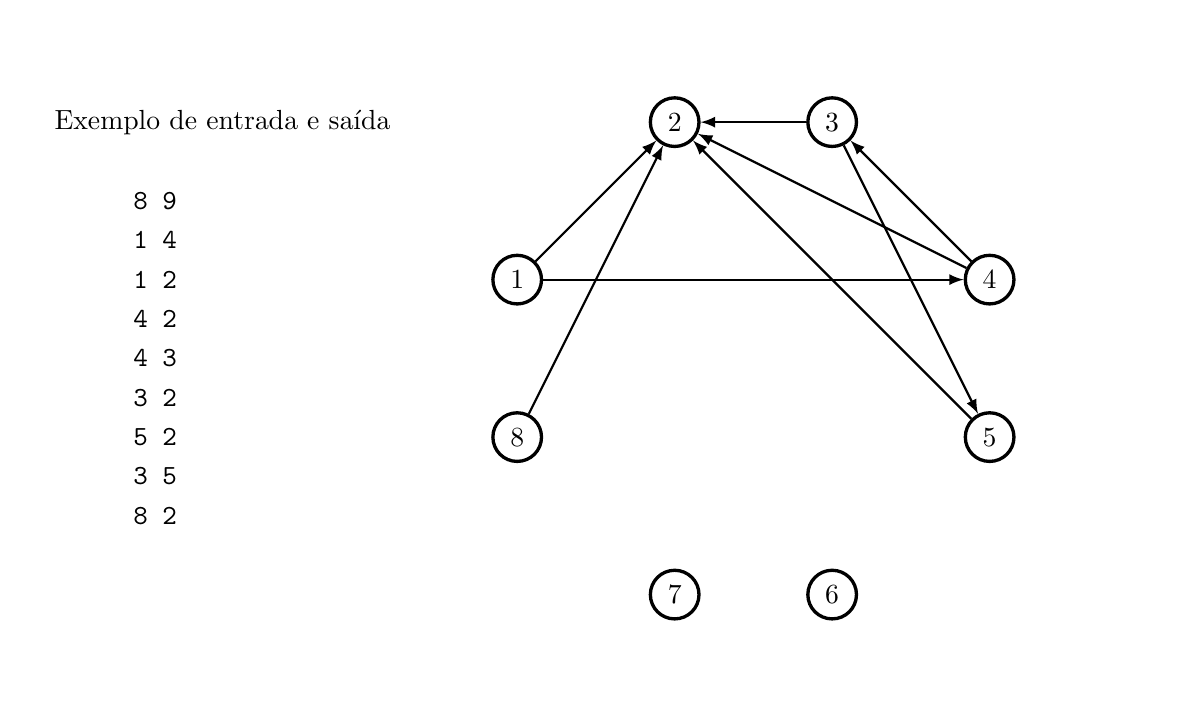
\begin{tikzpicture}
\node[draw,opacity=0] at (0, 0) {x};
\node[draw,opacity=0] at (14, 8) {x};

	\node[anchor=west] (header) at (0, 7.0) { \bbbold{Exemplo de entrada e saída} };


	\node[anchor=west] (line1) at (1.0, 6.0) { \bbtext{\texttt{8 9} } };







	\node[draw,very thick,circle] (node1) at (6.0, 5.0) { \bbtext{1} };

	\node[draw,very thick,circle] (node2) at (8.0, 7.0) { \bbtext{2} };

	\node[draw,very thick,circle] (node3) at (10.0, 7.0) { \bbtext{3} };

	\node[draw,very thick,circle] (node4) at (12.0, 5.0) { \bbtext{4} };

	\node[draw,very thick,circle] (node5) at (12.0, 3.0) { \bbtext{5} };

	\node[draw,very thick,circle] (node6) at (10.0, 1.0) { \bbtext{6} };

	\node[draw,very thick,circle] (node7) at (8.0, 1.0) { \bbtext{7} };

	\node[draw,very thick,circle] (node8) at (6.0, 3.0) { \bbtext{8} };




	\node[anchor=west] (line2) at (1.0, 5.5) { \bbtext{\texttt{1 4} } };






	\draw[thick,-latex](node1) to (node4);


	\node[anchor=west] (line3) at (1.0, 5.0) { \bbtext{\texttt{1 2} } };


	\draw[thick,-latex](node1) to (node2);


	\node[anchor=west] (line4) at (1.0, 4.5) { \bbtext{\texttt{4 2} } };


	\draw[thick,-latex](node4) to (node2);

	\node[anchor=west] (line5) at (1.0, 4.0) { \bbtext{\texttt{4 3} } };


	\draw[thick,-latex](node4) to (node3);


	\node[anchor=west] (line6) at (1.0, 3.5) { \bbtext{\texttt{3 2} } };


	\draw[thick,-latex](node3) to (node2);


	\node[anchor=west] (line7) at (1.0, 3.0) { \bbtext{\texttt{5 2} } };


	\draw[thick,-latex](node5) to (node2);


	\node[anchor=west] (line8) at (1.0, 2.5) { \bbtext{\texttt{3 5} } };


	\draw[thick,-latex](node3) to (node5);


	\node[anchor=west] (line9) at (1.0, 2.0) { \bbtext{\texttt{8 2} } };


	\draw[thick,-latex](node8) to (node2);

\end{tikzpicture}
\end{frame}
\begin{frame}[plain,t]
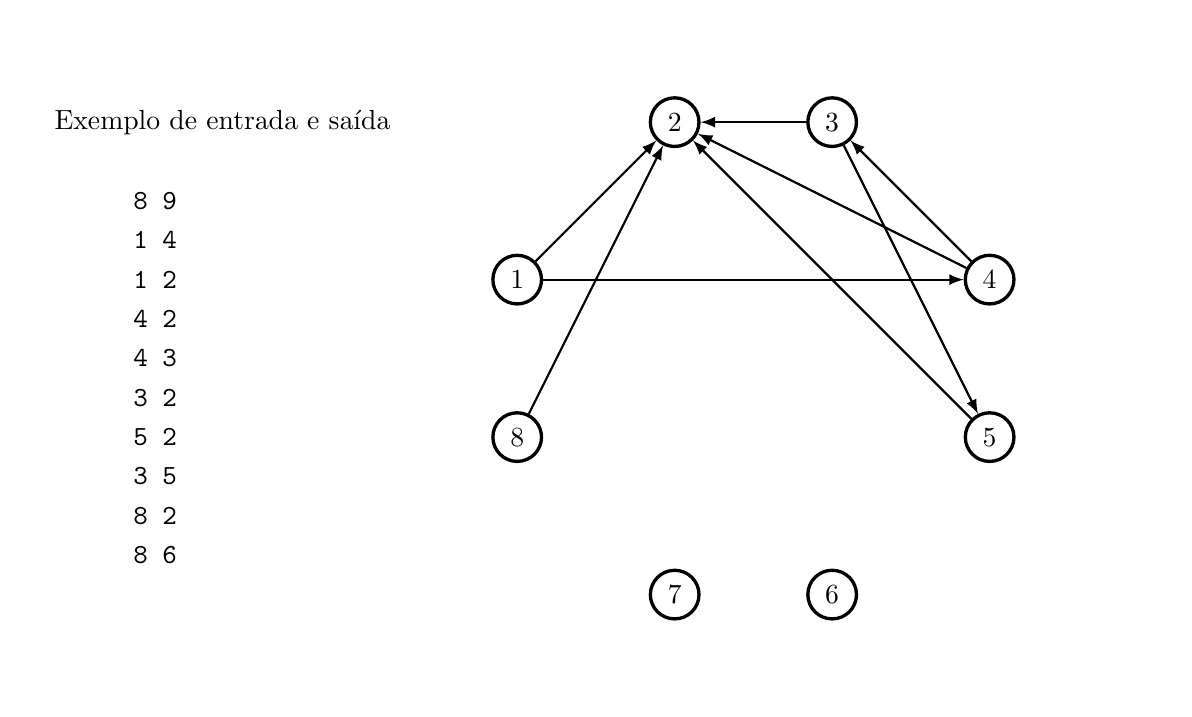
\begin{tikzpicture}
\node[draw,opacity=0] at (0, 0) {x};
\node[draw,opacity=0] at (14, 8) {x};

	\node[anchor=west] (header) at (0, 7.0) { \bbbold{Exemplo de entrada e saída} };


	\node[anchor=west] (line1) at (1.0, 6.0) { \bbtext{\texttt{8 9} } };







	\node[draw,very thick,circle] (node1) at (6.0, 5.0) { \bbtext{1} };

	\node[draw,very thick,circle] (node2) at (8.0, 7.0) { \bbtext{2} };

	\node[draw,very thick,circle] (node3) at (10.0, 7.0) { \bbtext{3} };

	\node[draw,very thick,circle] (node4) at (12.0, 5.0) { \bbtext{4} };

	\node[draw,very thick,circle] (node5) at (12.0, 3.0) { \bbtext{5} };

	\node[draw,very thick,circle] (node6) at (10.0, 1.0) { \bbtext{6} };

	\node[draw,very thick,circle] (node7) at (8.0, 1.0) { \bbtext{7} };

	\node[draw,very thick,circle] (node8) at (6.0, 3.0) { \bbtext{8} };




	\node[anchor=west] (line2) at (1.0, 5.5) { \bbtext{\texttt{1 4} } };






	\draw[thick,-latex](node1) to (node4);


	\node[anchor=west] (line3) at (1.0, 5.0) { \bbtext{\texttt{1 2} } };


	\draw[thick,-latex](node1) to (node2);


	\node[anchor=west] (line4) at (1.0, 4.5) { \bbtext{\texttt{4 2} } };


	\draw[thick,-latex](node4) to (node2);

	\node[anchor=west] (line5) at (1.0, 4.0) { \bbtext{\texttt{4 3} } };


	\draw[thick,-latex](node4) to (node3);


	\node[anchor=west] (line6) at (1.0, 3.5) { \bbtext{\texttt{3 2} } };


	\draw[thick,-latex](node3) to (node2);


	\node[anchor=west] (line7) at (1.0, 3.0) { \bbtext{\texttt{5 2} } };


	\draw[thick,-latex](node5) to (node2);


	\node[anchor=west] (line8) at (1.0, 2.5) { \bbtext{\texttt{3 5} } };


	\draw[thick,-latex](node3) to (node5);


	\node[anchor=west] (line9) at (1.0, 2.0) { \bbtext{\texttt{8 2} } };


	\draw[thick,-latex](node8) to (node2);


	\node[anchor=west] (line10) at (1.0, 1.5) { \bbtext{\texttt{8 6} } };

\end{tikzpicture}
\end{frame}
\begin{frame}[plain,t]
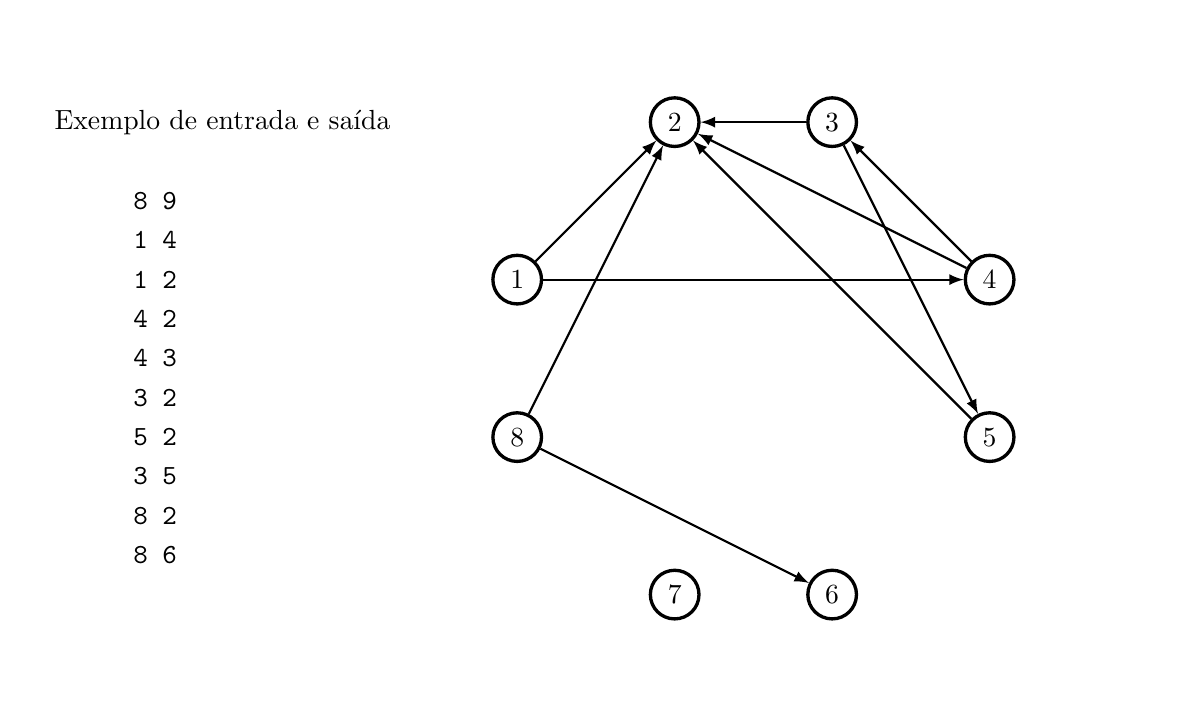
\begin{tikzpicture}
\node[draw,opacity=0] at (0, 0) {x};
\node[draw,opacity=0] at (14, 8) {x};

	\node[anchor=west] (header) at (0, 7.0) { \bbbold{Exemplo de entrada e saída} };


	\node[anchor=west] (line1) at (1.0, 6.0) { \bbtext{\texttt{8 9} } };







	\node[draw,very thick,circle] (node1) at (6.0, 5.0) { \bbtext{1} };

	\node[draw,very thick,circle] (node2) at (8.0, 7.0) { \bbtext{2} };

	\node[draw,very thick,circle] (node3) at (10.0, 7.0) { \bbtext{3} };

	\node[draw,very thick,circle] (node4) at (12.0, 5.0) { \bbtext{4} };

	\node[draw,very thick,circle] (node5) at (12.0, 3.0) { \bbtext{5} };

	\node[draw,very thick,circle] (node6) at (10.0, 1.0) { \bbtext{6} };

	\node[draw,very thick,circle] (node7) at (8.0, 1.0) { \bbtext{7} };

	\node[draw,very thick,circle] (node8) at (6.0, 3.0) { \bbtext{8} };




	\node[anchor=west] (line2) at (1.0, 5.5) { \bbtext{\texttt{1 4} } };






	\draw[thick,-latex](node1) to (node4);


	\node[anchor=west] (line3) at (1.0, 5.0) { \bbtext{\texttt{1 2} } };


	\draw[thick,-latex](node1) to (node2);


	\node[anchor=west] (line4) at (1.0, 4.5) { \bbtext{\texttt{4 2} } };


	\draw[thick,-latex](node4) to (node2);

	\node[anchor=west] (line5) at (1.0, 4.0) { \bbtext{\texttt{4 3} } };


	\draw[thick,-latex](node4) to (node3);


	\node[anchor=west] (line6) at (1.0, 3.5) { \bbtext{\texttt{3 2} } };


	\draw[thick,-latex](node3) to (node2);


	\node[anchor=west] (line7) at (1.0, 3.0) { \bbtext{\texttt{5 2} } };


	\draw[thick,-latex](node5) to (node2);


	\node[anchor=west] (line8) at (1.0, 2.5) { \bbtext{\texttt{3 5} } };


	\draw[thick,-latex](node3) to (node5);


	\node[anchor=west] (line9) at (1.0, 2.0) { \bbtext{\texttt{8 2} } };


	\draw[thick,-latex](node8) to (node2);


	\node[anchor=west] (line10) at (1.0, 1.5) { \bbtext{\texttt{8 6} } };


	\draw[thick,-latex](node8) to (node6);

\end{tikzpicture}
\end{frame}
\begin{frame}[plain,t]
\begin{tikzpicture}
\node[draw,opacity=0] at (0, 0) {x};
\node[draw,opacity=0] at (14, 8) {x};

	\node[anchor=west] (header) at (0, 7.0) { \bbbold{Exemplo de entrada e saída} };


	\node[anchor=west] (line1) at (1.0, 6.0) { \bbtext{\texttt{8 9} } };







	\node[draw,very thick,circle,fill=BBGreen] (node1) at (6.0, 5.0) { \bbtext{1} };

	\node[draw,very thick,circle] (node2) at (8.0, 7.0) { \bbtext{2} };

	\node[draw,very thick,circle] (node3) at (10.0, 7.0) { \bbtext{3} };

	\node[draw,very thick,circle] (node4) at (12.0, 5.0) { \bbtext{4} };

	\node[draw,very thick,circle] (node5) at (12.0, 3.0) { \bbtext{5} };

	\node[draw,very thick,circle] (node6) at (10.0, 1.0) { \bbtext{6} };

	\node[draw,very thick,circle,fill=BBGreen] (node7) at (8.0, 1.0) { \bbtext{7} };

	\node[draw,very thick,circle,fill=BBGreen] (node8) at (6.0, 3.0) { \bbtext{8} };




	\node[anchor=west] (line2) at (1.0, 5.5) { \bbtext{\texttt{1 4} } };






	\draw[thick,-latex](node1) to (node4);


	\node[anchor=west] (line3) at (1.0, 5.0) { \bbtext{\texttt{1 2} } };


	\draw[thick,-latex](node1) to (node2);


	\node[anchor=west] (line4) at (1.0, 4.5) { \bbtext{\texttt{4 2} } };


	\draw[thick,-latex](node4) to (node2);

	\node[anchor=west] (line5) at (1.0, 4.0) { \bbtext{\texttt{4 3} } };


	\draw[thick,-latex](node4) to (node3);


	\node[anchor=west] (line6) at (1.0, 3.5) { \bbtext{\texttt{3 2} } };


	\draw[thick,-latex](node3) to (node2);


	\node[anchor=west] (line7) at (1.0, 3.0) { \bbtext{\texttt{5 2} } };


	\draw[thick,-latex](node5) to (node2);


	\node[anchor=west] (line8) at (1.0, 2.5) { \bbtext{\texttt{3 5} } };


	\draw[thick,-latex](node3) to (node5);


	\node[anchor=west] (line9) at (1.0, 2.0) { \bbtext{\texttt{8 2} } };


	\draw[thick,-latex](node8) to (node2);


	\node[anchor=west] (line10) at (1.0, 1.5) { \bbtext{\texttt{8 6} } };


	\draw[thick,-latex](node8) to (node6);



\end{tikzpicture}
\end{frame}
\begin{frame}[plain,t]
\begin{tikzpicture}
\node[draw,opacity=0] at (0, 0) {x};
\node[draw,opacity=0] at (14, 8) {x};

	\node[anchor=west] (header) at (0, 7.0) { \bbbold{Exemplo de entrada e saída} };


	\node[anchor=west] (line1) at (1.0, 6.0) { \bbtext{\texttt{8 9} } };







	\node[draw,very thick,circle,fill=BBCyan] (node1) at (6.0, 5.0) { \bbtext{1} };

	\node[draw,very thick,circle] (node2) at (8.0, 7.0) { \bbtext{2} };

	\node[draw,very thick,circle] (node3) at (10.0, 7.0) { \bbtext{3} };

	\node[draw,very thick,circle] (node4) at (12.0, 5.0) { \bbtext{4} };

	\node[draw,very thick,circle] (node5) at (12.0, 3.0) { \bbtext{5} };

	\node[draw,very thick,circle] (node6) at (10.0, 1.0) { \bbtext{6} };

	\node[draw,very thick,circle,fill=BBGreen] (node7) at (8.0, 1.0) { \bbtext{7} };

	\node[draw,very thick,circle,fill=BBGreen] (node8) at (6.0, 3.0) { \bbtext{8} };




	\node[anchor=west] (line2) at (1.0, 5.5) { \bbtext{\texttt{1 4} } };






	\draw[thick,-latex](node1) to (node4);


	\node[anchor=west] (line3) at (1.0, 5.0) { \bbtext{\texttt{1 2} } };


	\draw[thick,-latex](node1) to (node2);


	\node[anchor=west] (line4) at (1.0, 4.5) { \bbtext{\texttt{4 2} } };


	\draw[thick,-latex](node4) to (node2);

	\node[anchor=west] (line5) at (1.0, 4.0) { \bbtext{\texttt{4 3} } };


	\draw[thick,-latex](node4) to (node3);


	\node[anchor=west] (line6) at (1.0, 3.5) { \bbtext{\texttt{3 2} } };


	\draw[thick,-latex](node3) to (node2);


	\node[anchor=west] (line7) at (1.0, 3.0) { \bbtext{\texttt{5 2} } };


	\draw[thick,-latex](node5) to (node2);


	\node[anchor=west] (line8) at (1.0, 2.5) { \bbtext{\texttt{3 5} } };


	\draw[thick,-latex](node3) to (node5);


	\node[anchor=west] (line9) at (1.0, 2.0) { \bbtext{\texttt{8 2} } };


	\draw[thick,-latex](node8) to (node2);


	\node[anchor=west] (line10) at (1.0, 1.5) { \bbtext{\texttt{8 6} } };


	\draw[thick,-latex](node8) to (node6);




\end{tikzpicture}
\end{frame}
\begin{frame}[plain,t]
\begin{tikzpicture}
\node[draw,opacity=0] at (0, 0) {x};
\node[draw,opacity=0] at (14, 8) {x};

	\node[anchor=west] (header) at (0, 7.0) { \bbbold{Exemplo de entrada e saída} };


	\node[anchor=west] (line1) at (1.0, 6.0) { \bbtext{\texttt{8 9} } };








	\node[draw,very thick,circle] (node2) at (8.0, 7.0) { \bbtext{2} };

	\node[draw,very thick,circle] (node3) at (10.0, 7.0) { \bbtext{3} };

	\node[draw,very thick,circle] (node4) at (12.0, 5.0) { \bbtext{4} };

	\node[draw,very thick,circle] (node5) at (12.0, 3.0) { \bbtext{5} };

	\node[draw,very thick,circle] (node6) at (10.0, 1.0) { \bbtext{6} };

	\node[draw,very thick,circle,fill=BBGreen] (node7) at (8.0, 1.0) { \bbtext{7} };

	\node[draw,very thick,circle,fill=BBGreen] (node8) at (6.0, 3.0) { \bbtext{8} };




	\node[anchor=west] (line2) at (1.0, 5.5) { \bbtext{\texttt{1 4} } };








	\node[anchor=west] (line3) at (1.0, 5.0) { \bbtext{\texttt{1 2} } };




	\node[anchor=west] (line4) at (1.0, 4.5) { \bbtext{\texttt{4 2} } };


	\draw[thick,-latex](node4) to (node2);

	\node[anchor=west] (line5) at (1.0, 4.0) { \bbtext{\texttt{4 3} } };


	\draw[thick,-latex](node4) to (node3);


	\node[anchor=west] (line6) at (1.0, 3.5) { \bbtext{\texttt{3 2} } };


	\draw[thick,-latex](node3) to (node2);


	\node[anchor=west] (line7) at (1.0, 3.0) { \bbtext{\texttt{5 2} } };


	\draw[thick,-latex](node5) to (node2);


	\node[anchor=west] (line8) at (1.0, 2.5) { \bbtext{\texttt{3 5} } };


	\draw[thick,-latex](node3) to (node5);


	\node[anchor=west] (line9) at (1.0, 2.0) { \bbtext{\texttt{8 2} } };


	\draw[thick,-latex](node8) to (node2);


	\node[anchor=west] (line10) at (1.0, 1.5) { \bbtext{\texttt{8 6} } };


	\draw[thick,-latex](node8) to (node6);





\end{tikzpicture}
\end{frame}
\begin{frame}[plain,t]
\begin{tikzpicture}
\node[draw,opacity=0] at (0, 0) {x};
\node[draw,opacity=0] at (14, 8) {x};

	\node[anchor=west] (header) at (0, 7.0) { \bbbold{Exemplo de entrada e saída} };


	\node[anchor=west] (line1) at (1.0, 6.0) { \bbtext{\texttt{8 9} } };








	\node[draw,very thick,circle] (node2) at (8.0, 7.0) { \bbtext{2} };

	\node[draw,very thick,circle] (node3) at (10.0, 7.0) { \bbtext{3} };

	\node[draw,very thick,circle,fill=BBGreen] (node4) at (12.0, 5.0) { \bbtext{4} };

	\node[draw,very thick,circle] (node5) at (12.0, 3.0) { \bbtext{5} };

	\node[draw,very thick,circle] (node6) at (10.0, 1.0) { \bbtext{6} };

	\node[draw,very thick,circle,fill=BBGreen] (node7) at (8.0, 1.0) { \bbtext{7} };

	\node[draw,very thick,circle,fill=BBGreen] (node8) at (6.0, 3.0) { \bbtext{8} };




	\node[anchor=west] (line2) at (1.0, 5.5) { \bbtext{\texttt{1 4} } };








	\node[anchor=west] (line3) at (1.0, 5.0) { \bbtext{\texttt{1 2} } };




	\node[anchor=west] (line4) at (1.0, 4.5) { \bbtext{\texttt{4 2} } };


	\draw[thick,-latex](node4) to (node2);

	\node[anchor=west] (line5) at (1.0, 4.0) { \bbtext{\texttt{4 3} } };


	\draw[thick,-latex](node4) to (node3);


	\node[anchor=west] (line6) at (1.0, 3.5) { \bbtext{\texttt{3 2} } };


	\draw[thick,-latex](node3) to (node2);


	\node[anchor=west] (line7) at (1.0, 3.0) { \bbtext{\texttt{5 2} } };


	\draw[thick,-latex](node5) to (node2);


	\node[anchor=west] (line8) at (1.0, 2.5) { \bbtext{\texttt{3 5} } };


	\draw[thick,-latex](node3) to (node5);


	\node[anchor=west] (line9) at (1.0, 2.0) { \bbtext{\texttt{8 2} } };


	\draw[thick,-latex](node8) to (node2);


	\node[anchor=west] (line10) at (1.0, 1.5) { \bbtext{\texttt{8 6} } };


	\draw[thick,-latex](node8) to (node6);






\end{tikzpicture}
\end{frame}
\begin{frame}[plain,t]
\begin{tikzpicture}
\node[draw,opacity=0] at (0, 0) {x};
\node[draw,opacity=0] at (14, 8) {x};

	\node[anchor=west] (header) at (0, 7.0) { \bbbold{Exemplo de entrada e saída} };


	\node[anchor=west] (line1) at (1.0, 6.0) { \bbtext{\texttt{8 9} } };








	\node[draw,very thick,circle] (node2) at (8.0, 7.0) { \bbtext{2} };

	\node[draw,very thick,circle] (node3) at (10.0, 7.0) { \bbtext{3} };

	\node[draw,very thick,circle,fill=BBCyan] (node4) at (12.0, 5.0) { \bbtext{4} };

	\node[draw,very thick,circle] (node5) at (12.0, 3.0) { \bbtext{5} };

	\node[draw,very thick,circle] (node6) at (10.0, 1.0) { \bbtext{6} };

	\node[draw,very thick,circle,fill=BBGreen] (node7) at (8.0, 1.0) { \bbtext{7} };

	\node[draw,very thick,circle,fill=BBGreen] (node8) at (6.0, 3.0) { \bbtext{8} };




	\node[anchor=west] (line2) at (1.0, 5.5) { \bbtext{\texttt{1 4} } };








	\node[anchor=west] (line3) at (1.0, 5.0) { \bbtext{\texttt{1 2} } };




	\node[anchor=west] (line4) at (1.0, 4.5) { \bbtext{\texttt{4 2} } };


	\draw[thick,-latex](node4) to (node2);

	\node[anchor=west] (line5) at (1.0, 4.0) { \bbtext{\texttt{4 3} } };


	\draw[thick,-latex](node4) to (node3);


	\node[anchor=west] (line6) at (1.0, 3.5) { \bbtext{\texttt{3 2} } };


	\draw[thick,-latex](node3) to (node2);


	\node[anchor=west] (line7) at (1.0, 3.0) { \bbtext{\texttt{5 2} } };


	\draw[thick,-latex](node5) to (node2);


	\node[anchor=west] (line8) at (1.0, 2.5) { \bbtext{\texttt{3 5} } };


	\draw[thick,-latex](node3) to (node5);


	\node[anchor=west] (line9) at (1.0, 2.0) { \bbtext{\texttt{8 2} } };


	\draw[thick,-latex](node8) to (node2);


	\node[anchor=west] (line10) at (1.0, 1.5) { \bbtext{\texttt{8 6} } };


	\draw[thick,-latex](node8) to (node6);







\end{tikzpicture}
\end{frame}
\begin{frame}[plain,t]
\begin{tikzpicture}
\node[draw,opacity=0] at (0, 0) {x};
\node[draw,opacity=0] at (14, 8) {x};

	\node[anchor=west] (header) at (0, 7.0) { \bbbold{Exemplo de entrada e saída} };


	\node[anchor=west] (line1) at (1.0, 6.0) { \bbtext{\texttt{8 9} } };








	\node[draw,very thick,circle] (node2) at (8.0, 7.0) { \bbtext{2} };

	\node[draw,very thick,circle] (node3) at (10.0, 7.0) { \bbtext{3} };


	\node[draw,very thick,circle] (node5) at (12.0, 3.0) { \bbtext{5} };

	\node[draw,very thick,circle] (node6) at (10.0, 1.0) { \bbtext{6} };

	\node[draw,very thick,circle,fill=BBGreen] (node7) at (8.0, 1.0) { \bbtext{7} };

	\node[draw,very thick,circle,fill=BBGreen] (node8) at (6.0, 3.0) { \bbtext{8} };




	\node[anchor=west] (line2) at (1.0, 5.5) { \bbtext{\texttt{1 4} } };








	\node[anchor=west] (line3) at (1.0, 5.0) { \bbtext{\texttt{1 2} } };




	\node[anchor=west] (line4) at (1.0, 4.5) { \bbtext{\texttt{4 2} } };



	\node[anchor=west] (line5) at (1.0, 4.0) { \bbtext{\texttt{4 3} } };




	\node[anchor=west] (line6) at (1.0, 3.5) { \bbtext{\texttt{3 2} } };


	\draw[thick,-latex](node3) to (node2);


	\node[anchor=west] (line7) at (1.0, 3.0) { \bbtext{\texttt{5 2} } };


	\draw[thick,-latex](node5) to (node2);


	\node[anchor=west] (line8) at (1.0, 2.5) { \bbtext{\texttt{3 5} } };


	\draw[thick,-latex](node3) to (node5);


	\node[anchor=west] (line9) at (1.0, 2.0) { \bbtext{\texttt{8 2} } };


	\draw[thick,-latex](node8) to (node2);


	\node[anchor=west] (line10) at (1.0, 1.5) { \bbtext{\texttt{8 6} } };


	\draw[thick,-latex](node8) to (node6);








\end{tikzpicture}
\end{frame}
\begin{frame}[plain,t]
\begin{tikzpicture}
\node[draw,opacity=0] at (0, 0) {x};
\node[draw,opacity=0] at (14, 8) {x};

	\node[anchor=west] (header) at (0, 7.0) { \bbbold{Exemplo de entrada e saída} };


	\node[anchor=west] (line1) at (1.0, 6.0) { \bbtext{\texttt{8 9} } };








	\node[draw,very thick,circle] (node2) at (8.0, 7.0) { \bbtext{2} };

	\node[draw,very thick,circle,fill=BBGreen] (node3) at (10.0, 7.0) { \bbtext{3} };


	\node[draw,very thick,circle] (node5) at (12.0, 3.0) { \bbtext{5} };

	\node[draw,very thick,circle] (node6) at (10.0, 1.0) { \bbtext{6} };

	\node[draw,very thick,circle,fill=BBGreen] (node7) at (8.0, 1.0) { \bbtext{7} };

	\node[draw,very thick,circle,fill=BBGreen] (node8) at (6.0, 3.0) { \bbtext{8} };




	\node[anchor=west] (line2) at (1.0, 5.5) { \bbtext{\texttt{1 4} } };








	\node[anchor=west] (line3) at (1.0, 5.0) { \bbtext{\texttt{1 2} } };




	\node[anchor=west] (line4) at (1.0, 4.5) { \bbtext{\texttt{4 2} } };



	\node[anchor=west] (line5) at (1.0, 4.0) { \bbtext{\texttt{4 3} } };




	\node[anchor=west] (line6) at (1.0, 3.5) { \bbtext{\texttt{3 2} } };


	\draw[thick,-latex](node3) to (node2);


	\node[anchor=west] (line7) at (1.0, 3.0) { \bbtext{\texttt{5 2} } };


	\draw[thick,-latex](node5) to (node2);


	\node[anchor=west] (line8) at (1.0, 2.5) { \bbtext{\texttt{3 5} } };


	\draw[thick,-latex](node3) to (node5);


	\node[anchor=west] (line9) at (1.0, 2.0) { \bbtext{\texttt{8 2} } };


	\draw[thick,-latex](node8) to (node2);


	\node[anchor=west] (line10) at (1.0, 1.5) { \bbtext{\texttt{8 6} } };


	\draw[thick,-latex](node8) to (node6);









\end{tikzpicture}
\end{frame}
\begin{frame}[plain,t]
\begin{tikzpicture}
\node[draw,opacity=0] at (0, 0) {x};
\node[draw,opacity=0] at (14, 8) {x};

	\node[anchor=west] (header) at (0, 7.0) { \bbbold{Exemplo de entrada e saída} };


	\node[anchor=west] (line1) at (1.0, 6.0) { \bbtext{\texttt{8 9} } };








	\node[draw,very thick,circle] (node2) at (8.0, 7.0) { \bbtext{2} };

	\node[draw,very thick,circle,fill=BBCyan] (node3) at (10.0, 7.0) { \bbtext{3} };


	\node[draw,very thick,circle] (node5) at (12.0, 3.0) { \bbtext{5} };

	\node[draw,very thick,circle] (node6) at (10.0, 1.0) { \bbtext{6} };

	\node[draw,very thick,circle,fill=BBGreen] (node7) at (8.0, 1.0) { \bbtext{7} };

	\node[draw,very thick,circle,fill=BBGreen] (node8) at (6.0, 3.0) { \bbtext{8} };




	\node[anchor=west] (line2) at (1.0, 5.5) { \bbtext{\texttt{1 4} } };








	\node[anchor=west] (line3) at (1.0, 5.0) { \bbtext{\texttt{1 2} } };




	\node[anchor=west] (line4) at (1.0, 4.5) { \bbtext{\texttt{4 2} } };



	\node[anchor=west] (line5) at (1.0, 4.0) { \bbtext{\texttt{4 3} } };




	\node[anchor=west] (line6) at (1.0, 3.5) { \bbtext{\texttt{3 2} } };


	\draw[thick,-latex](node3) to (node2);


	\node[anchor=west] (line7) at (1.0, 3.0) { \bbtext{\texttt{5 2} } };


	\draw[thick,-latex](node5) to (node2);


	\node[anchor=west] (line8) at (1.0, 2.5) { \bbtext{\texttt{3 5} } };


	\draw[thick,-latex](node3) to (node5);


	\node[anchor=west] (line9) at (1.0, 2.0) { \bbtext{\texttt{8 2} } };


	\draw[thick,-latex](node8) to (node2);


	\node[anchor=west] (line10) at (1.0, 1.5) { \bbtext{\texttt{8 6} } };


	\draw[thick,-latex](node8) to (node6);










\end{tikzpicture}
\end{frame}
\begin{frame}[plain,t]
\begin{tikzpicture}
\node[draw,opacity=0] at (0, 0) {x};
\node[draw,opacity=0] at (14, 8) {x};

	\node[anchor=west] (header) at (0, 7.0) { \bbbold{Exemplo de entrada e saída} };


	\node[anchor=west] (line1) at (1.0, 6.0) { \bbtext{\texttt{8 9} } };








	\node[draw,very thick,circle] (node2) at (8.0, 7.0) { \bbtext{2} };



	\node[draw,very thick,circle] (node5) at (12.0, 3.0) { \bbtext{5} };

	\node[draw,very thick,circle] (node6) at (10.0, 1.0) { \bbtext{6} };

	\node[draw,very thick,circle,fill=BBGreen] (node7) at (8.0, 1.0) { \bbtext{7} };

	\node[draw,very thick,circle,fill=BBGreen] (node8) at (6.0, 3.0) { \bbtext{8} };




	\node[anchor=west] (line2) at (1.0, 5.5) { \bbtext{\texttt{1 4} } };








	\node[anchor=west] (line3) at (1.0, 5.0) { \bbtext{\texttt{1 2} } };




	\node[anchor=west] (line4) at (1.0, 4.5) { \bbtext{\texttt{4 2} } };



	\node[anchor=west] (line5) at (1.0, 4.0) { \bbtext{\texttt{4 3} } };




	\node[anchor=west] (line6) at (1.0, 3.5) { \bbtext{\texttt{3 2} } };




	\node[anchor=west] (line7) at (1.0, 3.0) { \bbtext{\texttt{5 2} } };


	\draw[thick,-latex](node5) to (node2);


	\node[anchor=west] (line8) at (1.0, 2.5) { \bbtext{\texttt{3 5} } };




	\node[anchor=west] (line9) at (1.0, 2.0) { \bbtext{\texttt{8 2} } };


	\draw[thick,-latex](node8) to (node2);


	\node[anchor=west] (line10) at (1.0, 1.5) { \bbtext{\texttt{8 6} } };


	\draw[thick,-latex](node8) to (node6);











\end{tikzpicture}
\end{frame}
\begin{frame}[plain,t]
\begin{tikzpicture}
\node[draw,opacity=0] at (0, 0) {x};
\node[draw,opacity=0] at (14, 8) {x};

	\node[anchor=west] (header) at (0, 7.0) { \bbbold{Exemplo de entrada e saída} };


	\node[anchor=west] (line1) at (1.0, 6.0) { \bbtext{\texttt{8 9} } };








	\node[draw,very thick,circle] (node2) at (8.0, 7.0) { \bbtext{2} };



	\node[draw,very thick,circle,fill=BBGreen] (node5) at (12.0, 3.0) { \bbtext{5} };

	\node[draw,very thick,circle] (node6) at (10.0, 1.0) { \bbtext{6} };

	\node[draw,very thick,circle,fill=BBGreen] (node7) at (8.0, 1.0) { \bbtext{7} };

	\node[draw,very thick,circle,fill=BBGreen] (node8) at (6.0, 3.0) { \bbtext{8} };




	\node[anchor=west] (line2) at (1.0, 5.5) { \bbtext{\texttt{1 4} } };








	\node[anchor=west] (line3) at (1.0, 5.0) { \bbtext{\texttt{1 2} } };




	\node[anchor=west] (line4) at (1.0, 4.5) { \bbtext{\texttt{4 2} } };



	\node[anchor=west] (line5) at (1.0, 4.0) { \bbtext{\texttt{4 3} } };




	\node[anchor=west] (line6) at (1.0, 3.5) { \bbtext{\texttt{3 2} } };




	\node[anchor=west] (line7) at (1.0, 3.0) { \bbtext{\texttt{5 2} } };


	\draw[thick,-latex](node5) to (node2);


	\node[anchor=west] (line8) at (1.0, 2.5) { \bbtext{\texttt{3 5} } };




	\node[anchor=west] (line9) at (1.0, 2.0) { \bbtext{\texttt{8 2} } };


	\draw[thick,-latex](node8) to (node2);


	\node[anchor=west] (line10) at (1.0, 1.5) { \bbtext{\texttt{8 6} } };


	\draw[thick,-latex](node8) to (node6);












\end{tikzpicture}
\end{frame}
\begin{frame}[plain,t]
\begin{tikzpicture}
\node[draw,opacity=0] at (0, 0) {x};
\node[draw,opacity=0] at (14, 8) {x};

	\node[anchor=west] (header) at (0, 7.0) { \bbbold{Exemplo de entrada e saída} };


	\node[anchor=west] (line1) at (1.0, 6.0) { \bbtext{\texttt{8 9} } };








	\node[draw,very thick,circle] (node2) at (8.0, 7.0) { \bbtext{2} };



	\node[draw,very thick,circle,fill=BBCyan] (node5) at (12.0, 3.0) { \bbtext{5} };

	\node[draw,very thick,circle] (node6) at (10.0, 1.0) { \bbtext{6} };

	\node[draw,very thick,circle,fill=BBGreen] (node7) at (8.0, 1.0) { \bbtext{7} };

	\node[draw,very thick,circle,fill=BBGreen] (node8) at (6.0, 3.0) { \bbtext{8} };




	\node[anchor=west] (line2) at (1.0, 5.5) { \bbtext{\texttt{1 4} } };








	\node[anchor=west] (line3) at (1.0, 5.0) { \bbtext{\texttt{1 2} } };




	\node[anchor=west] (line4) at (1.0, 4.5) { \bbtext{\texttt{4 2} } };



	\node[anchor=west] (line5) at (1.0, 4.0) { \bbtext{\texttt{4 3} } };




	\node[anchor=west] (line6) at (1.0, 3.5) { \bbtext{\texttt{3 2} } };




	\node[anchor=west] (line7) at (1.0, 3.0) { \bbtext{\texttt{5 2} } };


	\draw[thick,-latex](node5) to (node2);


	\node[anchor=west] (line8) at (1.0, 2.5) { \bbtext{\texttt{3 5} } };




	\node[anchor=west] (line9) at (1.0, 2.0) { \bbtext{\texttt{8 2} } };


	\draw[thick,-latex](node8) to (node2);


	\node[anchor=west] (line10) at (1.0, 1.5) { \bbtext{\texttt{8 6} } };


	\draw[thick,-latex](node8) to (node6);













\end{tikzpicture}
\end{frame}
\begin{frame}[plain,t]
\begin{tikzpicture}
\node[draw,opacity=0] at (0, 0) {x};
\node[draw,opacity=0] at (14, 8) {x};

	\node[anchor=west] (header) at (0, 7.0) { \bbbold{Exemplo de entrada e saída} };


	\node[anchor=west] (line1) at (1.0, 6.0) { \bbtext{\texttt{8 9} } };








	\node[draw,very thick,circle] (node2) at (8.0, 7.0) { \bbtext{2} };




	\node[draw,very thick,circle] (node6) at (10.0, 1.0) { \bbtext{6} };

	\node[draw,very thick,circle,fill=BBGreen] (node7) at (8.0, 1.0) { \bbtext{7} };

	\node[draw,very thick,circle,fill=BBGreen] (node8) at (6.0, 3.0) { \bbtext{8} };




	\node[anchor=west] (line2) at (1.0, 5.5) { \bbtext{\texttt{1 4} } };








	\node[anchor=west] (line3) at (1.0, 5.0) { \bbtext{\texttt{1 2} } };




	\node[anchor=west] (line4) at (1.0, 4.5) { \bbtext{\texttt{4 2} } };



	\node[anchor=west] (line5) at (1.0, 4.0) { \bbtext{\texttt{4 3} } };




	\node[anchor=west] (line6) at (1.0, 3.5) { \bbtext{\texttt{3 2} } };




	\node[anchor=west] (line7) at (1.0, 3.0) { \bbtext{\texttt{5 2} } };




	\node[anchor=west] (line8) at (1.0, 2.5) { \bbtext{\texttt{3 5} } };




	\node[anchor=west] (line9) at (1.0, 2.0) { \bbtext{\texttt{8 2} } };


	\draw[thick,-latex](node8) to (node2);


	\node[anchor=west] (line10) at (1.0, 1.5) { \bbtext{\texttt{8 6} } };


	\draw[thick,-latex](node8) to (node6);














\end{tikzpicture}
\end{frame}
\begin{frame}[plain,t]
\begin{tikzpicture}
\node[draw,opacity=0] at (0, 0) {x};
\node[draw,opacity=0] at (14, 8) {x};

	\node[anchor=west] (header) at (0, 7.0) { \bbbold{Exemplo de entrada e saída} };


	\node[anchor=west] (line1) at (1.0, 6.0) { \bbtext{\texttt{8 9} } };








	\node[draw,very thick,circle] (node2) at (8.0, 7.0) { \bbtext{2} };




	\node[draw,very thick,circle] (node6) at (10.0, 1.0) { \bbtext{6} };

	\node[draw,very thick,circle,fill=BBCyan] (node7) at (8.0, 1.0) { \bbtext{7} };

	\node[draw,very thick,circle,fill=BBGreen] (node8) at (6.0, 3.0) { \bbtext{8} };




	\node[anchor=west] (line2) at (1.0, 5.5) { \bbtext{\texttt{1 4} } };








	\node[anchor=west] (line3) at (1.0, 5.0) { \bbtext{\texttt{1 2} } };




	\node[anchor=west] (line4) at (1.0, 4.5) { \bbtext{\texttt{4 2} } };



	\node[anchor=west] (line5) at (1.0, 4.0) { \bbtext{\texttt{4 3} } };




	\node[anchor=west] (line6) at (1.0, 3.5) { \bbtext{\texttt{3 2} } };




	\node[anchor=west] (line7) at (1.0, 3.0) { \bbtext{\texttt{5 2} } };




	\node[anchor=west] (line8) at (1.0, 2.5) { \bbtext{\texttt{3 5} } };




	\node[anchor=west] (line9) at (1.0, 2.0) { \bbtext{\texttt{8 2} } };


	\draw[thick,-latex](node8) to (node2);


	\node[anchor=west] (line10) at (1.0, 1.5) { \bbtext{\texttt{8 6} } };


	\draw[thick,-latex](node8) to (node6);















\end{tikzpicture}
\end{frame}
\begin{frame}[plain,t]
\begin{tikzpicture}
\node[draw,opacity=0] at (0, 0) {x};
\node[draw,opacity=0] at (14, 8) {x};

	\node[anchor=west] (header) at (0, 7.0) { \bbbold{Exemplo de entrada e saída} };


	\node[anchor=west] (line1) at (1.0, 6.0) { \bbtext{\texttt{8 9} } };








	\node[draw,very thick,circle] (node2) at (8.0, 7.0) { \bbtext{2} };




	\node[draw,very thick,circle] (node6) at (10.0, 1.0) { \bbtext{6} };


	\node[draw,very thick,circle,fill=BBGreen] (node8) at (6.0, 3.0) { \bbtext{8} };




	\node[anchor=west] (line2) at (1.0, 5.5) { \bbtext{\texttt{1 4} } };








	\node[anchor=west] (line3) at (1.0, 5.0) { \bbtext{\texttt{1 2} } };




	\node[anchor=west] (line4) at (1.0, 4.5) { \bbtext{\texttt{4 2} } };



	\node[anchor=west] (line5) at (1.0, 4.0) { \bbtext{\texttt{4 3} } };




	\node[anchor=west] (line6) at (1.0, 3.5) { \bbtext{\texttt{3 2} } };




	\node[anchor=west] (line7) at (1.0, 3.0) { \bbtext{\texttt{5 2} } };




	\node[anchor=west] (line8) at (1.0, 2.5) { \bbtext{\texttt{3 5} } };




	\node[anchor=west] (line9) at (1.0, 2.0) { \bbtext{\texttt{8 2} } };


	\draw[thick,-latex](node8) to (node2);


	\node[anchor=west] (line10) at (1.0, 1.5) { \bbtext{\texttt{8 6} } };


	\draw[thick,-latex](node8) to (node6);
















\end{tikzpicture}
\end{frame}
\begin{frame}[plain,t]
\begin{tikzpicture}
\node[draw,opacity=0] at (0, 0) {x};
\node[draw,opacity=0] at (14, 8) {x};

	\node[anchor=west] (header) at (0, 7.0) { \bbbold{Exemplo de entrada e saída} };


	\node[anchor=west] (line1) at (1.0, 6.0) { \bbtext{\texttt{8 9} } };








	\node[draw,very thick,circle] (node2) at (8.0, 7.0) { \bbtext{2} };




	\node[draw,very thick,circle] (node6) at (10.0, 1.0) { \bbtext{6} };


	\node[draw,very thick,circle,fill=BBCyan] (node8) at (6.0, 3.0) { \bbtext{8} };




	\node[anchor=west] (line2) at (1.0, 5.5) { \bbtext{\texttt{1 4} } };








	\node[anchor=west] (line3) at (1.0, 5.0) { \bbtext{\texttt{1 2} } };




	\node[anchor=west] (line4) at (1.0, 4.5) { \bbtext{\texttt{4 2} } };



	\node[anchor=west] (line5) at (1.0, 4.0) { \bbtext{\texttt{4 3} } };




	\node[anchor=west] (line6) at (1.0, 3.5) { \bbtext{\texttt{3 2} } };




	\node[anchor=west] (line7) at (1.0, 3.0) { \bbtext{\texttt{5 2} } };




	\node[anchor=west] (line8) at (1.0, 2.5) { \bbtext{\texttt{3 5} } };




	\node[anchor=west] (line9) at (1.0, 2.0) { \bbtext{\texttt{8 2} } };


	\draw[thick,-latex](node8) to (node2);


	\node[anchor=west] (line10) at (1.0, 1.5) { \bbtext{\texttt{8 6} } };


	\draw[thick,-latex](node8) to (node6);

















\end{tikzpicture}
\end{frame}
\begin{frame}[plain,t]
\begin{tikzpicture}
\node[draw,opacity=0] at (0, 0) {x};
\node[draw,opacity=0] at (14, 8) {x};

	\node[anchor=west] (header) at (0, 7.0) { \bbbold{Exemplo de entrada e saída} };


	\node[anchor=west] (line1) at (1.0, 6.0) { \bbtext{\texttt{8 9} } };








	\node[draw,very thick,circle] (node2) at (8.0, 7.0) { \bbtext{2} };




	\node[draw,very thick,circle] (node6) at (10.0, 1.0) { \bbtext{6} };






	\node[anchor=west] (line2) at (1.0, 5.5) { \bbtext{\texttt{1 4} } };








	\node[anchor=west] (line3) at (1.0, 5.0) { \bbtext{\texttt{1 2} } };




	\node[anchor=west] (line4) at (1.0, 4.5) { \bbtext{\texttt{4 2} } };



	\node[anchor=west] (line5) at (1.0, 4.0) { \bbtext{\texttt{4 3} } };




	\node[anchor=west] (line6) at (1.0, 3.5) { \bbtext{\texttt{3 2} } };




	\node[anchor=west] (line7) at (1.0, 3.0) { \bbtext{\texttt{5 2} } };




	\node[anchor=west] (line8) at (1.0, 2.5) { \bbtext{\texttt{3 5} } };




	\node[anchor=west] (line9) at (1.0, 2.0) { \bbtext{\texttt{8 2} } };




	\node[anchor=west] (line10) at (1.0, 1.5) { \bbtext{\texttt{8 6} } };




















\end{tikzpicture}
\end{frame}
\begin{frame}[plain,t]
\begin{tikzpicture}
\node[draw,opacity=0] at (0, 0) {x};
\node[draw,opacity=0] at (14, 8) {x};

	\node[anchor=west] (header) at (0, 7.0) { \bbbold{Exemplo de entrada e saída} };


	\node[anchor=west] (line1) at (1.0, 6.0) { \bbtext{\texttt{8 9} } };








	\node[draw,very thick,circle,fill=BBGreen] (node2) at (8.0, 7.0) { \bbtext{2} };




	\node[draw,very thick,circle,fill=BBGreen] (node6) at (10.0, 1.0) { \bbtext{6} };






	\node[anchor=west] (line2) at (1.0, 5.5) { \bbtext{\texttt{1 4} } };








	\node[anchor=west] (line3) at (1.0, 5.0) { \bbtext{\texttt{1 2} } };




	\node[anchor=west] (line4) at (1.0, 4.5) { \bbtext{\texttt{4 2} } };



	\node[anchor=west] (line5) at (1.0, 4.0) { \bbtext{\texttt{4 3} } };




	\node[anchor=west] (line6) at (1.0, 3.5) { \bbtext{\texttt{3 2} } };




	\node[anchor=west] (line7) at (1.0, 3.0) { \bbtext{\texttt{5 2} } };




	\node[anchor=west] (line8) at (1.0, 2.5) { \bbtext{\texttt{3 5} } };




	\node[anchor=west] (line9) at (1.0, 2.0) { \bbtext{\texttt{8 2} } };




	\node[anchor=west] (line10) at (1.0, 1.5) { \bbtext{\texttt{8 6} } };





















\end{tikzpicture}
\end{frame}
\begin{frame}[plain,t]
\begin{tikzpicture}
\node[draw,opacity=0] at (0, 0) {x};
\node[draw,opacity=0] at (14, 8) {x};

	\node[anchor=west] (header) at (0, 7.0) { \bbbold{Exemplo de entrada e saída} };


	\node[anchor=west] (line1) at (1.0, 6.0) { \bbtext{\texttt{8 9} } };








	\node[draw,very thick,circle,fill=BBCyan] (node2) at (8.0, 7.0) { \bbtext{2} };




	\node[draw,very thick,circle,fill=BBGreen] (node6) at (10.0, 1.0) { \bbtext{6} };






	\node[anchor=west] (line2) at (1.0, 5.5) { \bbtext{\texttt{1 4} } };








	\node[anchor=west] (line3) at (1.0, 5.0) { \bbtext{\texttt{1 2} } };




	\node[anchor=west] (line4) at (1.0, 4.5) { \bbtext{\texttt{4 2} } };



	\node[anchor=west] (line5) at (1.0, 4.0) { \bbtext{\texttt{4 3} } };




	\node[anchor=west] (line6) at (1.0, 3.5) { \bbtext{\texttt{3 2} } };




	\node[anchor=west] (line7) at (1.0, 3.0) { \bbtext{\texttt{5 2} } };




	\node[anchor=west] (line8) at (1.0, 2.5) { \bbtext{\texttt{3 5} } };




	\node[anchor=west] (line9) at (1.0, 2.0) { \bbtext{\texttt{8 2} } };




	\node[anchor=west] (line10) at (1.0, 1.5) { \bbtext{\texttt{8 6} } };





















\end{tikzpicture}
\end{frame}
\begin{frame}[plain,t]
\begin{tikzpicture}
\node[draw,opacity=0] at (0, 0) {x};
\node[draw,opacity=0] at (14, 8) {x};

	\node[anchor=west] (header) at (0, 7.0) { \bbbold{Exemplo de entrada e saída} };


	\node[anchor=west] (line1) at (1.0, 6.0) { \bbtext{\texttt{8 9} } };












	\node[draw,very thick,circle,fill=BBGreen] (node6) at (10.0, 1.0) { \bbtext{6} };






	\node[anchor=west] (line2) at (1.0, 5.5) { \bbtext{\texttt{1 4} } };








	\node[anchor=west] (line3) at (1.0, 5.0) { \bbtext{\texttt{1 2} } };




	\node[anchor=west] (line4) at (1.0, 4.5) { \bbtext{\texttt{4 2} } };



	\node[anchor=west] (line5) at (1.0, 4.0) { \bbtext{\texttt{4 3} } };




	\node[anchor=west] (line6) at (1.0, 3.5) { \bbtext{\texttt{3 2} } };




	\node[anchor=west] (line7) at (1.0, 3.0) { \bbtext{\texttt{5 2} } };




	\node[anchor=west] (line8) at (1.0, 2.5) { \bbtext{\texttt{3 5} } };




	\node[anchor=west] (line9) at (1.0, 2.0) { \bbtext{\texttt{8 2} } };




	\node[anchor=west] (line10) at (1.0, 1.5) { \bbtext{\texttt{8 6} } };






















\end{tikzpicture}
\end{frame}
\begin{frame}[plain,t]
\begin{tikzpicture}
\node[draw,opacity=0] at (0, 0) {x};
\node[draw,opacity=0] at (14, 8) {x};

	\node[anchor=west] (header) at (0, 7.0) { \bbbold{Exemplo de entrada e saída} };


	\node[anchor=west] (line1) at (1.0, 6.0) { \bbtext{\texttt{8 9} } };












	\node[draw,very thick,circle,fill=BBCyan] (node6) at (10.0, 1.0) { \bbtext{6} };






	\node[anchor=west] (line2) at (1.0, 5.5) { \bbtext{\texttt{1 4} } };








	\node[anchor=west] (line3) at (1.0, 5.0) { \bbtext{\texttt{1 2} } };




	\node[anchor=west] (line4) at (1.0, 4.5) { \bbtext{\texttt{4 2} } };



	\node[anchor=west] (line5) at (1.0, 4.0) { \bbtext{\texttt{4 3} } };




	\node[anchor=west] (line6) at (1.0, 3.5) { \bbtext{\texttt{3 2} } };




	\node[anchor=west] (line7) at (1.0, 3.0) { \bbtext{\texttt{5 2} } };




	\node[anchor=west] (line8) at (1.0, 2.5) { \bbtext{\texttt{3 5} } };




	\node[anchor=west] (line9) at (1.0, 2.0) { \bbtext{\texttt{8 2} } };




	\node[anchor=west] (line10) at (1.0, 1.5) { \bbtext{\texttt{8 6} } };






















\end{tikzpicture}
\end{frame}
\begin{frame}[plain,t]
\begin{tikzpicture}
\node[draw,opacity=0] at (0, 0) {x};
\node[draw,opacity=0] at (14, 8) {x};

	\node[anchor=west] (header) at (0, 7.0) { \bbbold{Exemplo de entrada e saída} };


	\node[anchor=west] (line1) at (1.0, 6.0) { \bbtext{\texttt{8 9} } };


















	\node[anchor=west] (line2) at (1.0, 5.5) { \bbtext{\texttt{1 4} } };








	\node[anchor=west] (line3) at (1.0, 5.0) { \bbtext{\texttt{1 2} } };




	\node[anchor=west] (line4) at (1.0, 4.5) { \bbtext{\texttt{4 2} } };



	\node[anchor=west] (line5) at (1.0, 4.0) { \bbtext{\texttt{4 3} } };




	\node[anchor=west] (line6) at (1.0, 3.5) { \bbtext{\texttt{3 2} } };




	\node[anchor=west] (line7) at (1.0, 3.0) { \bbtext{\texttt{5 2} } };




	\node[anchor=west] (line8) at (1.0, 2.5) { \bbtext{\texttt{3 5} } };




	\node[anchor=west] (line9) at (1.0, 2.0) { \bbtext{\texttt{8 2} } };




	\node[anchor=west] (line10) at (1.0, 1.5) { \bbtext{\texttt{8 6} } };























\end{tikzpicture}
\end{frame}
\begin{frame}[plain,t]
\begin{tikzpicture}
\node[draw,opacity=0] at (0, 0) {x};
\node[draw,opacity=0] at (14, 8) {x};

	\node[anchor=west] (header) at (0, 7.0) { \bbbold{Exemplo de entrada e saída} };


	\node[anchor=west] (line1) at (1.0, 6.0) { \bbtext{\texttt{8 9} } };


	\draw[->,color=BBBlack,very thick,-latex] (2.25, 2.5) to  (3.25, 2.5);

	\node[anchor=west] (r) at (3.5, 2.5) { \footnotesize \bboutput{1 4 3 5 7 8 2 6} };















	\node[anchor=west] (line2) at (1.0, 5.5) { \bbtext{\texttt{1 4} } };








	\node[anchor=west] (line3) at (1.0, 5.0) { \bbtext{\texttt{1 2} } };




	\node[anchor=west] (line4) at (1.0, 4.5) { \bbtext{\texttt{4 2} } };



	\node[anchor=west] (line5) at (1.0, 4.0) { \bbtext{\texttt{4 3} } };




	\node[anchor=west] (line6) at (1.0, 3.5) { \bbtext{\texttt{3 2} } };




	\node[anchor=west] (line7) at (1.0, 3.0) { \bbtext{\texttt{5 2} } };




	\node[anchor=west] (line8) at (1.0, 2.5) { \bbtext{\texttt{3 5} } };




	\node[anchor=west] (line9) at (1.0, 2.0) { \bbtext{\texttt{8 2} } };




	\node[anchor=west] (line10) at (1.0, 1.5) { \bbtext{\texttt{8 6} } };

























\end{tikzpicture}
\end{frame}
\begin{frame}[plain,t]
\begin{tikzpicture}
\node[draw,opacity=0] at (0, 0) {x};
\node[draw,opacity=0] at (14, 8) {x};

	\node[anchor=west] (header) at (0, 7.0) { \bbbold{Exemplo de entrada e saída} };

\end{tikzpicture}
\end{frame}
\begin{frame}[plain,t]
\begin{tikzpicture}
\node[draw,opacity=0] at (0, 0) {x};
\node[draw,opacity=0] at (14, 8) {x};

	\node[anchor=west] (header) at (0, 7.0) { \bbbold{Exemplo de entrada e saída} };


	\node[anchor=west] (line1) at (1.0, 6.0) { \bbtext{\texttt{2 2} } };

\end{tikzpicture}
\end{frame}
\begin{frame}[plain,t]
\begin{tikzpicture}
\node[draw,opacity=0] at (0, 0) {x};
\node[draw,opacity=0] at (14, 8) {x};

	\node[anchor=west] (header) at (0, 7.0) { \bbbold{Exemplo de entrada e saída} };


	\node[anchor=west] (line1) at (1.0, 6.0) { \bbtext{\texttt{2 2} } };


	\node[draw,very thick,circle] (a) at (7.0, 4.0) { \bbtext{1} };

	\node[draw,very thick,circle] (b) at (12.0, 4.0) { \bbtext{2} };

\end{tikzpicture}
\end{frame}
\begin{frame}[plain,t]
\begin{tikzpicture}
\node[draw,opacity=0] at (0, 0) {x};
\node[draw,opacity=0] at (14, 8) {x};

	\node[anchor=west] (header) at (0, 7.0) { \bbbold{Exemplo de entrada e saída} };


	\node[anchor=west] (line1) at (1.0, 6.0) { \bbtext{\texttt{2 2} } };


	\node[draw,very thick,circle] (a) at (7.0, 4.0) { \bbtext{1} };

	\node[draw,very thick,circle] (b) at (12.0, 4.0) { \bbtext{2} };


	\node[anchor=west] (line2) at (1.0, 5.5) { \bbtext{\texttt{1 2} } };

\end{tikzpicture}
\end{frame}
\begin{frame}[plain,t]
\begin{tikzpicture}
\node[draw,opacity=0] at (0, 0) {x};
\node[draw,opacity=0] at (14, 8) {x};

	\node[anchor=west] (header) at (0, 7.0) { \bbbold{Exemplo de entrada e saída} };


	\node[anchor=west] (line1) at (1.0, 6.0) { \bbtext{\texttt{2 2} } };


	\node[draw,very thick,circle] (a) at (7.0, 4.0) { \bbtext{1} };

	\node[draw,very thick,circle] (b) at (12.0, 4.0) { \bbtext{2} };


	\node[anchor=west] (line2) at (1.0, 5.5) { \bbtext{\texttt{1 2} } };


	\draw[thick,-latex](a) to [bend left] (b);

\end{tikzpicture}
\end{frame}
\begin{frame}[plain,t]
\begin{tikzpicture}
\node[draw,opacity=0] at (0, 0) {x};
\node[draw,opacity=0] at (14, 8) {x};

	\node[anchor=west] (header) at (0, 7.0) { \bbbold{Exemplo de entrada e saída} };


	\node[anchor=west] (line1) at (1.0, 6.0) { \bbtext{\texttt{2 2} } };


	\node[draw,very thick,circle] (a) at (7.0, 4.0) { \bbtext{1} };

	\node[draw,very thick,circle] (b) at (12.0, 4.0) { \bbtext{2} };


	\node[anchor=west] (line2) at (1.0, 5.5) { \bbtext{\texttt{1 2} } };


	\draw[thick,-latex](a) to [bend left] (b);


	\node[anchor=west] (line3) at (1.0, 5.0) { \bbtext{\texttt{2 1 } } };

\end{tikzpicture}
\end{frame}
\begin{frame}[plain,t]
\begin{tikzpicture}
\node[draw,opacity=0] at (0, 0) {x};
\node[draw,opacity=0] at (14, 8) {x};

	\node[anchor=west] (header) at (0, 7.0) { \bbbold{Exemplo de entrada e saída} };


	\node[anchor=west] (line1) at (1.0, 6.0) { \bbtext{\texttt{2 2} } };


	\node[draw,very thick,circle] (a) at (7.0, 4.0) { \bbtext{1} };

	\node[draw,very thick,circle] (b) at (12.0, 4.0) { \bbtext{2} };


	\node[anchor=west] (line2) at (1.0, 5.5) { \bbtext{\texttt{1 2} } };


	\draw[thick,-latex](a) to [bend left] (b);


	\node[anchor=west] (line3) at (1.0, 5.0) { \bbtext{\texttt{2 1 } } };


	\draw[thick,-latex](b) to [bend left] (a);

\end{tikzpicture}
\end{frame}
\begin{frame}[plain,t]
\begin{tikzpicture}
\node[draw,opacity=0] at (0, 0) {x};
\node[draw,opacity=0] at (14, 8) {x};

	\node[anchor=west] (header) at (0, 7.0) { \bbbold{Exemplo de entrada e saída} };


	\node[anchor=west] (line1) at (1.0, 6.0) { \bbtext{\texttt{2 2} } };


	\node[draw,very thick,circle] (a) at (7.0, 4.0) { \bbtext{1} };

	\node[draw,very thick,circle] (b) at (12.0, 4.0) { \bbtext{2} };


	\node[anchor=west] (line2) at (1.0, 5.5) { \bbtext{\texttt{1 2} } };


	\draw[thick,-latex](a) to [bend left] (b);


	\node[anchor=west] (line3) at (1.0, 5.0) { \bbtext{\texttt{2 1 } } };


	\draw[thick,-latex](b) to [bend left] (a);

	\node[] (r) at (1.45, 3.5) { \footnotesize \bboutput{Sandro fails.} };

	\draw[color=BBBlack,very thick,-latex] (1.45, 4.75) to  (1.45, 3.75);

\end{tikzpicture}
\end{frame}
\begin{frame}[plain,t]
\begin{tikzpicture}
\node[draw,opacity=0] at (0, 0) {x};
\node[draw,opacity=0] at (14, 8) {x};

	\node[anchor=west] (title) at (0.0, 7.0) { \Large \bbbold{Solução} };
\end{tikzpicture}
\end{frame}
\begin{frame}[plain,t]
\begin{tikzpicture}
\node[draw,opacity=0] at (0, 0) {x};
\node[draw,opacity=0] at (14, 8) {x};

	\node[anchor=west] (title) at (0.0, 7.0) { \Large \bbbold{Solução} };

	\node[anchor=west] (a) at (1.0, 6.0) { $\star$ \bbtext{Sandro será capaz de cumprir suas tarefas apenas se elas puderem ser} };

	\node[anchor=west] (a1) at (0.5, 5.5) { \bbtext{ordenadas de tal forma que as prioridades sejam respeitadas} };

\end{tikzpicture}
\end{frame}
\begin{frame}[plain,t]
\begin{tikzpicture}
\node[draw,opacity=0] at (0, 0) {x};
\node[draw,opacity=0] at (14, 8) {x};

	\node[anchor=west] (title) at (0.0, 7.0) { \Large \bbbold{Solução} };

	\node[anchor=west] (a) at (1.0, 6.0) { $\star$ \bbtext{Sandro será capaz de cumprir suas tarefas apenas se elas puderem ser} };

	\node[anchor=west] (a1) at (0.5, 5.5) { \bbtext{ordenadas de tal forma que as prioridades sejam respeitadas} };


	\node[anchor=west] (b) at (1.0, 4.5) { $\star$ \bbtext{Em outras palavras, há solução apenas se existe uma ordenação topológica} };

\end{tikzpicture}
\end{frame}
\begin{frame}[plain,t]
\begin{tikzpicture}
\node[draw,opacity=0] at (0, 0) {x};
\node[draw,opacity=0] at (14, 8) {x};

	\node[anchor=west] (title) at (0.0, 7.0) { \Large \bbbold{Solução} };

	\node[anchor=west] (a) at (1.0, 6.0) { $\star$ \bbtext{Sandro será capaz de cumprir suas tarefas apenas se elas puderem ser} };

	\node[anchor=west] (a1) at (0.5, 5.5) { \bbtext{ordenadas de tal forma que as prioridades sejam respeitadas} };


	\node[anchor=west] (b) at (1.0, 4.5) { $\star$ \bbtext{Em outras palavras, há solução apenas se existe uma ordenação topológica} };


	\node[anchor=west] (c) at (1.0, 3.5) { $\star$ \bbtext{Se o grafo tem um ou mais ciclos, a resposta é \bboutput{Sandro fails.}} };

\end{tikzpicture}
\end{frame}
\begin{frame}[plain,t]
\begin{tikzpicture}
\node[draw,opacity=0] at (0, 0) {x};
\node[draw,opacity=0] at (14, 8) {x};

	\node[anchor=west] (title) at (0.0, 7.0) { \Large \bbbold{Solução} };

	\node[anchor=west] (a) at (1.0, 6.0) { $\star$ \bbtext{Sandro será capaz de cumprir suas tarefas apenas se elas puderem ser} };

	\node[anchor=west] (a1) at (0.5, 5.5) { \bbtext{ordenadas de tal forma que as prioridades sejam respeitadas} };


	\node[anchor=west] (b) at (1.0, 4.5) { $\star$ \bbtext{Em outras palavras, há solução apenas se existe uma ordenação topológica} };


	\node[anchor=west] (c) at (1.0, 3.5) { $\star$ \bbtext{Se o grafo tem um ou mais ciclos, a resposta é \bboutput{Sandro fails.}} };


	\node[anchor=west] (d) at (1.0, 2.5) { $\star$ \bbtext{O problema pede, na saída, uma ordenação específica} };

\end{tikzpicture}
\end{frame}
\begin{frame}[plain,t]
\begin{tikzpicture}
\node[draw,opacity=0] at (0, 0) {x};
\node[draw,opacity=0] at (14, 8) {x};

	\node[anchor=west] (title) at (0.0, 7.0) { \Large \bbbold{Solução} };

	\node[anchor=west] (a) at (1.0, 6.0) { $\star$ \bbtext{Sandro será capaz de cumprir suas tarefas apenas se elas puderem ser} };

	\node[anchor=west] (a1) at (0.5, 5.5) { \bbtext{ordenadas de tal forma que as prioridades sejam respeitadas} };


	\node[anchor=west] (b) at (1.0, 4.5) { $\star$ \bbtext{Em outras palavras, há solução apenas se existe uma ordenação topológica} };


	\node[anchor=west] (c) at (1.0, 3.5) { $\star$ \bbtext{Se o grafo tem um ou mais ciclos, a resposta é \bboutput{Sandro fails.}} };


	\node[anchor=west] (d) at (1.0, 2.5) { $\star$ \bbtext{O problema pede, na saída, uma ordenação específica} };


	\node[anchor=west] (e) at (1.0, 1.5) { $\star$ \bbtext{Esta ordenação pode ser obtida se a fila do algoritmo de Kahn for} };

	\node[anchor=west] (e1) at (0.5, 1.0) { \bbtext{substituída por uma \bbenglish{min heap}} };


\end{tikzpicture}
\end{frame}
\begin{frame}[plain,t]

\inputsnippet{cpp}{11}{29}{codes/TOPOSORT.cpp}

\end{frame}
\begin{frame}[plain,t]

\inputsnippet{cpp}{31}{42}{codes/TOPOSORT.cpp}


\end{frame}
\end{document}
